\documentclass[11pt]{article}
\usepackage{xcolor}
\usepackage{textcomp}
\usepackage{hyperref}
\usepackage{subcaption}
\usepackage{graphicx}
\usepackage{wrapfig}
\usepackage{amsmath}
\usepackage{array}
\usepackage{afterpage}
\usepackage{helvet}
\usepackage[style=numeric-comp, sorting=none, backend=biber]{biblatex}
\addbibresource{refs.bib}
\usepackage[a4paper, margin=1in, footskip=0.25in]{geometry}

\def\tableComp{
	{\sffamily
	\footnotesize
	\centering
	% \label{table:strategies_overview}
	\begin{tabular}{ p{\wTstr}|p{\wTstr}|p{\wTstr}|p{\wTstr} }
		& \hfil $\theta$ = 0 & \hfil $\theta$ = 5 & \hfil $\theta$ = 10 \\ 
		\hline
		Random-Discrete & \hfil AlwaysDefect & \hfil (50\% 0.00\textbar 1.00) & \hfil AlwaysCooperate \\  
		\hline
		Random-Continuous & \hfil AlwaysNeutral & \hfil (50\% 0.25\textbar 0.75) & \hfil (50\% 0.00\textbar 1.00) \\
		\hline
		Always-Same & \hfil AlwaysDefect & \hfil AlwaysNeutral & \hfil AlwaysCooperate \\
		\hline
		Adapt-Discrete & \hfil AlwaysCooperate & \hfil (rounded TFT) & \hfil (rounded overshot TFT)\\
		\hline
		Adapt-Continuous & \hfil AlwaysNeutral & \hfil TFT & \hfil (overshot TFT)
	\end{tabular}
	}
}

\newcommand\emptypage{
    \null
    \thispagestyle{empty}
    \addtocounter{page}{-1}
    \newpage
    }

\makeatletter
\renewcommand{\listoffigures}{%
  \subsection*{\listfigurename}%
  \textit{Figure \ref{fig:heatmaps} was generated by ChatGPT; all the other figures are self-created.}
  \@starttoc{lof}%
}
\renewcommand{\listoftables}{%
  \subsection*{\listtablename}%
  \textit{Table \ref{table:strategies_overview} is self-created.}
  \@starttoc{lot}%
}
\makeatother

\defbibheading{bibliography}[\refname]{}
% relative path to images directory
% \graphicspath{ {./plots/} }
\newcommand{\round}[1]{\ensuremath{\lfloor#1\rceil}}
\setcounter{page}{0}
\renewcommand{\contentsname}{Table of Contents}
% \newcommand{\multiply}[2]{\the\numexpr#1*#2\relax}
% TODO: multiply for title format 

% make captions of figures cursive
\DeclareCaptionFormat{custom}
{
    \textbf{#1#2}\textit{\small #3}
}
\captionsetup{format=custom}
% \captionsetup{singlelinecheck=false}

\newcommand{\vdist}{3}
\newcommand{\dvdist}{\the\numexpr2*\vdist\relax}

\title{
	\textbf{Counteracting Erratic Behaviour:}\\
	\textbf{A Game-Theoretical Analysis of Parametrised Strategies}\\[\dvdist ex]
	\Large{High-School Thesis}\\
	\Large{(Maturaarbeit)}\\[\vdist ex]
	\Large{Mathematical-Computational}\\
	\Large{Analysis}\\[\vdist ex]
	\Large{Author:}\\
	\Large{Adrian Hossner}\\[3\vdist ex]
	\begin{flushleft}
		\begin{tabular}{>{\raggedright\arraybackslash}p{6cm} >{\raggedright\arraybackslash}p{5cm}}
			\Large{Supervisor: } & \Large{Dr. Geoffrey Ostrin}\\[\vdist ex]
			\Large{Submission Date: } & \Large{September 7, 2025}\\[\vdist ex]
			\Large{School: } & \Large{Gymnasium Thun}\\[\vdist ex]
			\Large{Word Count (Sections 1-6): } & \Large{8166}\\[\vdist ex]
		\end{tabular}
	\end{flushleft}
}
\date{ } % display no date

\begin{document}

% make text never surpass the margin
\sloppy

\maketitle
\pagenumbering{gobble}

\newpage

\emptypage

\pagenumbering{arabic}

\section*{Abstract}
This high-school thesis addresses the politically and socially relevant question of how to best counteract erratic behaviour.
To this end, game theory is used as a theoretical framework, in particular the Prisoner's Dilemma game.
In its extended version of the iterated continuous Prisoner's Dilemma, two persons repeatedly play against each other and win or lose points depending on how they mutually treated each other in the previous round.
A discrete and a continuous random strategy are chosen as erratic behaviours, which compete against each other as well as against a rigid strategy and a discrete and a continuous version of an adaptive strategy.
All strategies are parametrised (from 0 to 10) in terms of the rigour with which the respective strategy is pursued.
The results are presented in the form of individual absolute- and relative-gain plots as well as an overall-gain plot that reflects the benefit achieved jointly by both players.
On the one hand, the mathematical-computational analysis reveals surprising details, which are discussed in detail under the headings of shallow randomness, dispersion and risk, threshold values for discrete adaptations, and dynamics of continuous adaptations.
On the other hand, when examining the interactions in terms of gains accumulated against randomness, no strong strategy could be identified that successfully counteracts unpredictable behaviour while maximising relative- and overall-gain values simultaneously.
In the case of encountering erratic behaviour, the summarising recommendation is that, if one's own advantage is emphasised, cooperation should be completely rejected, while some cooperation should be offered if one is dealing with an at least partially rational interaction partner.

\newpage

\section*{Preface}
The present thesis has been written in times of global uncertainty.
At least partially, this is ascribed to a more or less erratic behaviour of political leaders---as a prime example the 47\textsuperscript{th} President of the U.S.A. Donald J. Trump.
When discussing this issue among my family and friends, a water-polo team member of mine drew my attention to the fact that this problem of erratic behaviour could be mathematically modelled by means of game theory.
Of particular interest in this context would be the so-called 'Prisoner's Dilemma'.
This game has been popularised in the 'A Beautiful Mind' film that narrates a story about the famous mathematician John Forbes Nash.
The opportunity of combining my politically-social concerns with my subject-related interests in Computer Science and Mathematics captivated me immediately.
Hence, I was more than delighted that my school teacher Mr Ostrin accepted my request to serve as a supervisor of a related high-school thesis.\\
\indent Since then, Mr Ostrin has been always approachable and an extremely valuable supporter of my work.
Likewise, I am grateful for all the help I have received from my parents, be it as inspiring discussants, critical proofreaders, or supportive coaches when I was temporarily stuck in problems. Many thanks from the bottom of my heart!


\newpage

\tableofcontents
\newpage

\section{Introduction} \label{sec:intro}
On August 9-10, 2025, the 'Süddeutsche Zeitung' (p.~20) reported on massive irritations of the incumbent Federal President of Switzerland Karin Keller-Sutter, stemming from the ongoing tariff dispute with the United States of America.
In this context, the U.S. President's unpredictable character is perceived as particularly bothersome.
Consequently, the question arises how to successfully counteract such erratic behaviour on the political stage.\\
\indent Game theory offers a powerful framework for studying human decision making, for the issue sketched above, especially in the form of the Prisoner's Dilemma (PD) game.
When translating 'erratic behaviour' as pursuing a random PD strategy, the resulting leading question of the present thesis would aim at identifying strategies that prove to be effective countermeasures against randomness.
In addition, it seems interesting to ask whether gradations of erratic behaviour matter, meaning that a game-theoretical computational analysis would be required to allow parametrisation.
Finally---and in sharp contrast to an 'America First' ideology---it appears worthwhile to investigate not only superiority over opponents but the overall gain collectively achieved as well.\\
\indent The leading question derived in the present introduction (Section \ref{sec:intro}) will be explored below in five consecutive steps: After relevant theoretical foundations have been laid (Section \ref{sec:theoretical_found}), applied methods and implementational specifications of the computational analysis will be presented (Section \ref{sec:methods_and_implementation}).
Subsequently, the obtained results will be described (Section \ref{sec:results}) and discussed (Section \ref{sec:discussion}). 
The thesis will be rounded off with a conclusion and outlook that refers back to the leading question just formulated (Section \ref{sec:conclusion}) and will be supplemented by a source list (Section \ref{sec:sources}), an appendix (\ref{sec:appendices}) and a declaration of integrity (\ref{sec:declaration_of_integrity}).

\section{Theoretical Foundations} \label{sec:theoretical_found}

To grasp the game-theoretical approach pursued in this thesis, it is necessary to first understand the underlying key concepts. 
The most important ones, being the PD (2.1), the introduction of iterations as an extension (2.2) and the approach of submitting continuous values (2.3).
Finally, further PD variants will be mentioned (2.4) and relevant information of published researches will be provided (2.5).
Excellent overviews are available in standard encyclopedia, from which the information reported in 2.1–2.4 was compiled, in particular the \textit{International Encyclopedia of the Social and Behavioral Sciences} \cite{RC15} and the \textit{Stanford Encyclopedia of Philosophy} \cite{Kuh25}.

\subsection{Prisoner's Dilemma}
		
The PD is a famous model in game theory. 
To understand the dilemma, a proper context has to be established:
Two persons are arrested and sued for having committed a crime jointly.
There is yet, however, insufficient evidence to imprison the two suspects.
Despite not having enough prove, the police interrogates them separately without giving them a chance to coordinate beforehand.
The suspects receive two options.
On the one hand, they can confess that the other suspect was involved in the crime. 
On the other hand, they have the right to remain silent.
In case mutual trust and thus no confession took place, both separately receive an imprisonment of three years.
If both confess, either obtains ten years in prison.
However, if one chooses to confess while the other remains silent, the informer is sentenced to only one year in prison, whereas the betrayed is punished with 25 years.
Remaining silent is considered as cooperation, whereby defection is the opposite, meaning breaking confidence. 
The following matrix visualises the pay-offs in this game in a comprehensive way, with C representing cooperation and D corresponding to defection:

% specific pay-off matrix
\begin{center}
\begin{tabular}{ c|c|c }
   & C & D \\ 
   \hline
 C & 3, 3 & 25, 1\\  
   \hline
 D & 1, 25 & 10, 10
\end{tabular}
\end{center}

\noindent
The dilemma consists of the following:
The act of defecting is tempting since there is a chance of avoiding a long sentence.
However, it is then also possible to receive a punishment of ten years in prison depending on the confederate's decision.
Nevertheless, this outcome---which could have been avoided if both had remained silent and thus obtained a reward of three easy surmountable years in confinement---is the most likely result, as the temptation to defect is simply too great.
Additionally, the possibility of becoming the sucker in this game forces the player to consider trust as the deciding factor.
As trust is bound to be unreliable, defection is the more reasonable choice.
The PD thus composes a one-time interaction from a mathematical and analytical perspective. 
In a more general form, the variables can be described as Reward ($R$), Sucker's pay-off ($S$), Temptation ($T$), and Punishment ($P$) as follows:

% general pay-off matrix
\begin{center}
\begin{tabular}{ c|c|c }
   & C & D \\ 
   \hline
 C & R, R & S, T\\  
   \hline
 D & T, S & P, P
\end{tabular}
\end{center}

\noindent The pay-offs in the matrix can be altered as long as the following inequalities stay valid:

\begin{equation}
	T < R < P < S
	\label{eq:TRPS}
\end{equation}

\subsection{Iterated Prisoner's Dilemma}
		
The Iterated Prisoner's Dilemma (IPD) extends the PD as the game is played multiple times sequentially. 
To refer to the number of rounds played, $n$ is used as the denotation. 
The gained pay-offs are accumulated over the last $n-k$ rounds where $k$ represents the current round.
A player's strategy can be based on the entire history of the previous PDs to generate the decision for the next round.
These decisions can be calculated using conditions and probabilities that are applied to the given data.
The prison analogy is changed from minimising years in prison to maximising one's points.
Thus, the pay-off matrix must be altered accordingly.
In particular, the following inequalities need to be satisfied:
%
% \begin{center}
% \begin{tabular}{ c|c|c }
%    & C & D \\ 
%    \hline
%  C & R, R & S, T\\  
%    \hline
%  D & T, S & P, P
% \end{tabular}
% \end{center}

\begin{equation}
T > R > P > S
\end{equation}
An additional inequality is necessary to avoid receiving greater pay-offs by coordinated alternation of cooperation and defection ($T + S$) than continued mutual cooperation ($2 R$):
\begin{equation}\label{eq:AvGrPa}
2R > T + S
\end{equation}

\noindent
In the IPD, mutual cooperation yields long-term benefits since playing cooperation increases trust.
The maximum pay-off, however, can only be achieved by exploitation ($p_{\mathrm{max}} = n T$).
Because persistent defection leads to mutual defection as a response, the attainment of this maximum value is highly unlikely.

% A problem arises in the last round.
% Since cooperation is only played to conserve trust, the reasonable action in the last round is to defect as trust has no use beyond the game.
% If both strategies act rational, mutual defection will be played in the last round.
% And because both are aware of this fact, there is no logical reason to cooperate the second last round.
% This will end up in an inductive defection behaviour for both strategies the whole game.
% So, to prevent constant mutual defection, the number of rounds played is an information that needs to be hidden from both strategies.
% As a consequence of that, $n$ is a random number whose limits can be defined.\\
% This extension of the PD allows to simulate a relationship of two individuals.
%
\subsection{Iterated Continuous Prisoner's Dilemma} \label{sec:iterated_continuous_prisoners_dilemma}

In the Iterated Continuous Prisoner's Dilemma (ICPD), strategies are not limited to either cooperate or defect.
Instead, the players can choose any level of cooperation between 0 (defect) and 1 (cooperate).
This cooperation level is called investment or contribution.
The continuous form offers enhanced precision and mathematical applicability.
% One would suspect a very similar pay-off system to the iterated variant.
% In the discrete version, it looked like this:
%
% \begin{center}
% \begin{tabular}{ c c }
% Pay-off Player A & Pay-off Player B\\
% \begin{tabular}{ c|c|c }
%    & $C_A$ & $D_A$ \\ 
%    \hline
%  $C_B$ & 3 & 5\\  
%    \hline
%  $D_B$ & 0 & 1
% \end{tabular}
% &
% \begin{tabular}{ c|c|c }
%    & $C_A$ & $D_A$ \\ 
%    \hline
%  $C_B$ & 3 & 0\\  
%    \hline
%  $D_B$ & 5 & 1
% \end{tabular}
% \end{tabular}
% \end{center}

To include continuous values in the ICPD, a mathematical procedure can be applied to the discrete version of the matrix, namely bilinear interpolation.
This will establish a field that can be represented by colour grades, a heat map as depicted in Figure \ref{fig:heatmaps}.

\begin{figure}[h]
	\centering
	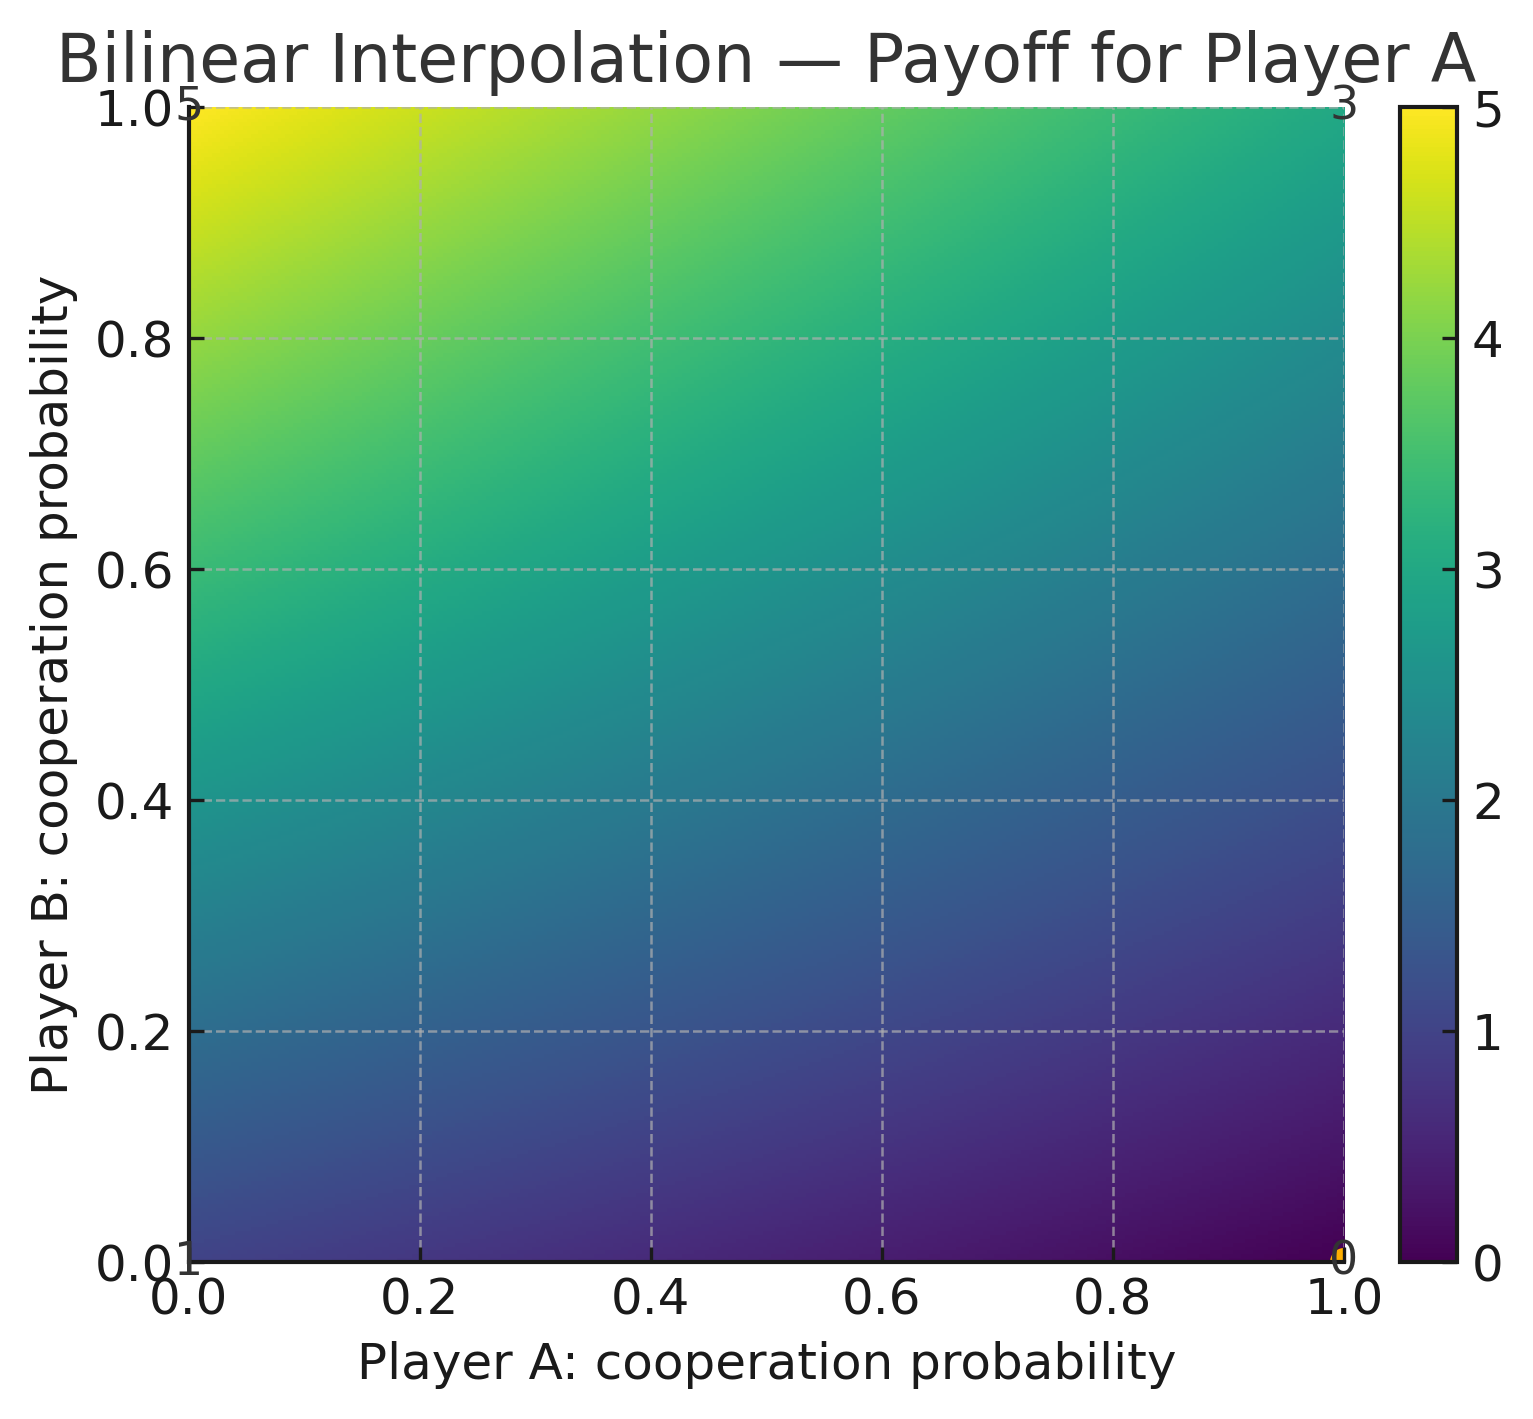
\includegraphics[width=0.45\textwidth]{images/pd_heatmap_A}\hfill
	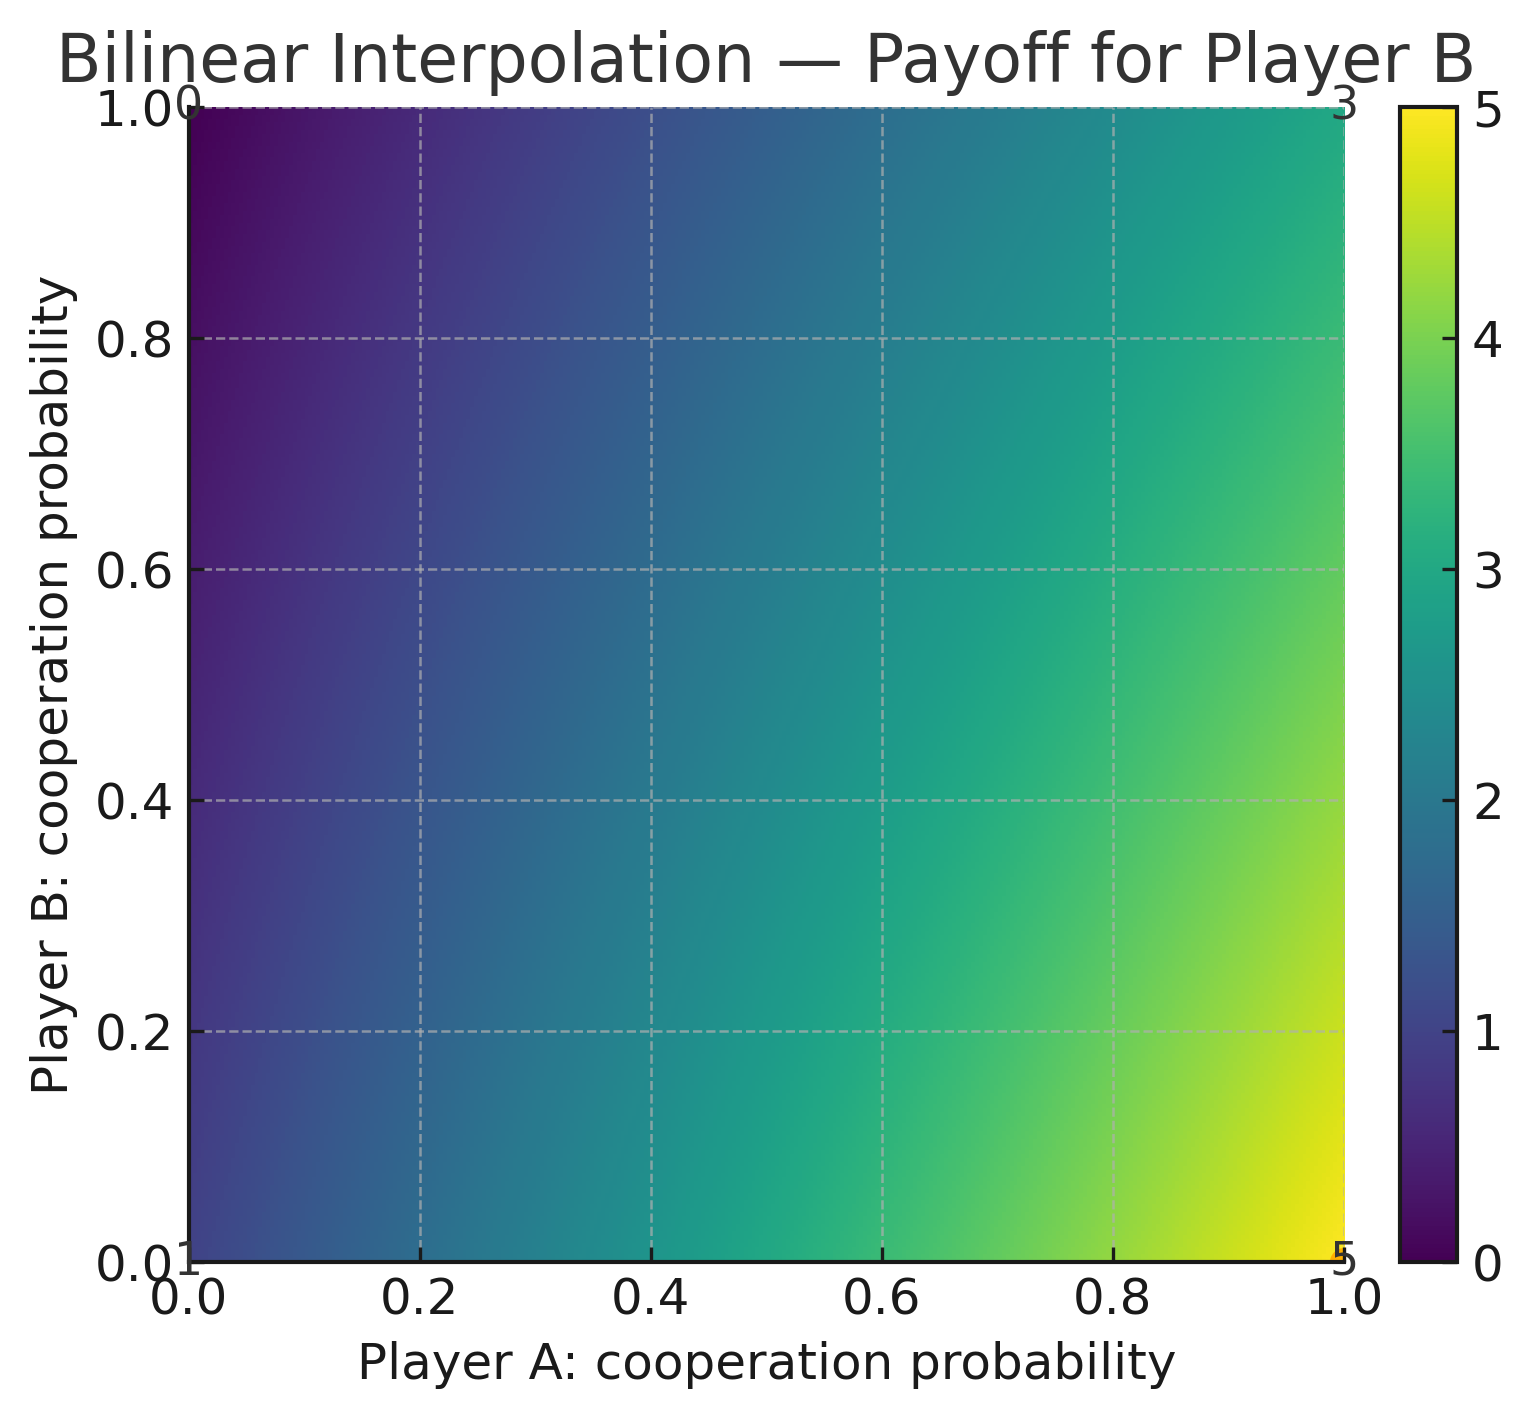
\includegraphics[width=0.45\textwidth]{images/pd_heatmap_B}
	\caption{Pay-off heat maps in the ICPD for player A (left) and player B (right).}
	\label{fig:heatmaps}
\end{figure}

% I used ChatGPT-o4 to generate these heat maps.
% It generated them using these functions:
%
% $$U_A = (1-x)(1-y)R_A + (1-x)yS_A + x(1-y)T_A + xyP_A$$
% $$U_B = (1-x)(1-y)R_B + (1-x)yS_B + x(1-y)T_B + xyP_B$$
%
% These functions are applied to every point on the map.
% The variable x is the investment of strategy A and y is the investment of strategy B.
For reason of simplifying analysability, this pay-off system can be expressed in the following equations \cite[cf.][p.~259]{LB07}:

\begin{equation}
	p_A = y - c x + c
	\label{eq:payoff_A}
\end{equation}
\begin{equation}
	p_B = x - c y + c
	\label{eq:payoff_B}
\end{equation}

\noindent
In these equations, $p_A$ and $p_B$ are the pay-offs of strategy A and B, respectively.
$x$ is the investment of strategy A and $y$ is that of strategy B.
The coefficient $c$ ranges, as well as $x$ and $y$, from 0 to 1 (inclusively) and describes the cost of cooperation.
The pay-off is highly affected by the opponent's investment.
Only a fraction of one's own contribution is subtracted, $c$ being the coefficient.
Consequently, the minimum pay-off would then be $-c$.
However, to avoid negative pay-offs and enhance comprehensibility of results achieved, a third addend is appended in the present thesis, namely $c$.
So, the least points that can be gained is 0 while the maximal points that can be earned by exploitation is $1 + c$.

% Let's see if the principles of the initial PD are still valid.
% It is better for one to defect (submit a 0) to get rid of the subtraction.
% And it is better for the strategy if the opponent's cooperates.
% If both defect, one gets zero points.
% If both cooperate, both get one point.
% If, however, one strategy exploits the opponent, meaning it defects while the other cooperates, it will get the maximum points being 1.
% The opponent would then get $-c$ points.
% This is the least one can receive.

		% 0 to 1 rather than cooperation or defection\\
		% Pay-off system\\ % https://www.sciencedirect.com/science/article/pii/S0022519306004255?casa_token=hIA0lYvzjf8AAAAA:Up2uQ89wotaLz7s1R0dM2FK7SaulAo40wIM-BdM9yooZ8uJeRL6mPs-K55dPNGs4XkcclNVjDQ#aep-section-id24
		% more accurate\\
		% more complex, generates more data \textrightarrow more insightful\\

\subsection{Further Variants}

There exist several extensions of the PD, one of which is noise, meaning that investments are altered with a certain probability.
This noise is introduced to simulate potential misunderstandings.
Another advancement is the alternating form.
In this variant, investments are contributed by the players in succession rather than concurrently as in the conventional simultaneous model.
Finally, the evolutionary PD game surveys the success of strategies in a world where natural selection takes place.
This implies that losing strategies vanish, while successful ones replicate and ultimately survive a PD tournament.
However, since the ICPD---as introduced above---offers a promising and apparently sufficient framework for approaching the leading question, those further variants can be disregarded in the present thesis.

% \subsection{Noise}
%
% Noise in the ICPD is the equivalent to miscommunication or misunderstanding in the real world.
% In this variant of the PD, noise is essential to trigger interesting outcomes.
% When a game of the ICPD is started and two strategies who start with a full investment, many strategies only respond with full investments.
% So noise is necessary to trigger continuous investments. 
% Without noise, in many cases, the ICPD would be equivalent to the IPD.
%
% 		% sometimes necessary to trigger continuous investments\\
% 		% simulates misunderstandings\\
%
% \subsection{Simultaneous vs Alternating}
%
% Two main differences can be seen when simulating an iterated variant of the PD.
% On one hand there is the simultaneous form whereby the strategies submit their contribution at the same time.
% On the other hand, there is the alternating form in which on e strategy submits its contribution and the other strategy can respond to this contribution is that round.
% Since the alternating form gives and advantage to the strategy which is allowed to respond, this only makes things more complicated than necessary.
% So, this analysis is only dedicated to the simultaneous form.
\subsection{Scientific Findings} \label{sec:scientific_findings}
In the context of the PD, erratic behaviour might be characterised best as 'random strategy'.
To retrieve the most important scientific findings on this topic, a literature search was conducted on \url{scholar.google.com} with the search terms 'Prisoner's Dilemma' and 'random strategy' (for details see Appendix \ref{sec:appendices}).
A criterion-based process of stepwise reduction of the initially found 650 hits finally resulted in eight publications of particular relevance.

Interestingly, a random strategy was already included in the first conducted PD tournament organised by Axelrod and Hamilton \cite{AH81}.
Their main finding is that a simple Tit-for-Tat strategy (TFT: “start with a C, and then use your co-players previous move”, \cite{NS93}) won over all other strategies.
In his review on PD studies, Brembs \cite[p.~14]{Bre96} highlights as one of the “most important advancements in the game-theoretical work on different aspects of the game” the turn from deterministic to stochastic variants.
In this context, Nowak and Sigmund \cite[p.~56]{NS93} argue that “occasional mistakes between two TFT players cause long runs of mutual backbiting.” They thus introduce a so-called Pavlov strategy, which “cooperates if and only if both players opted for the same alternative in the previous move (…). Thus Pavlov (…) can correct mistakes.” 
Building on this, Kraines and Kraines \cite[p.~112]{KK93} demonstrate that “Pavlov will exploit (…) random strategies” in the discrete IPD game.
Even further optimisations were suggested by Hauert and Stenull \cite{HS02} in terms of adaptive strategies and by Hao, Li and Zhou \cite{HLZ18} for ways of determining the opponent’s maximum and minimum gain.
Jurišić, Kermek and Konecki \cite{JKK12} report in their review on repetitions of Axelrod’s tournament in 2004 and 2005 on a successful Omega TFT strategy that always defects as soon as a certain randomness threshold is crossed by the opponent. 
Finally, Mathieu and Delahaye \cite[pp.~4, 5]{MD17} introduce new strategies that perform better than probabilistic or random strategies, namely soft\_majo (“begins by cooperating and cooperates as long as the number of times the opponent has cooperated is greater that or equal to the number of times it has defected”) and gradual (“cooperates on the first move, then defect $n$ times after $n$\textsuperscript{th} defections of its opponent, and calms down with 2 cooperations”).

Despite the scientific progress that becomes obvious with this short summary, it should be first noted that all of the retrieved articles refer to an overall success in a tournament with multiple strategies rather than a specific advantage over a random opponent. 
Second, success is understood as outperforming the opponent without also considering the overall gain of both players.
Third, the discrete variant of the IPD is used, which does not include certain gradations of randomness. 
The last-mentioned point is strikingly corroborated by the fact that an additionally conducted scholar.google.com search with the terms 'continuous Prisoner's Dilemma' and 'random strategy' delivered three hits only, all of which are irrelevant for the present topic \cite{Ash08, HLD13, Lei11}. 
It seems thus fair to conclude that a mathematical simulation of a competition of continuously parametrised strategies against strategies of graded randomness with a particular focus also on both players’ overall gain is worth pursuing further in the present thesis. 

\section{Methods and Implementation} \label{sec:methods_and_implementation}

To answer the leading question, it is necessary to develop an overarching study design (\ref{sec:study_design}), to specify the parametrised strategies that will be pursued in the ICPD (\ref{sec:implemented_strategies}), and to determine details of the implementation in terms of IT (\ref{sec:implementational_details}).

\subsection{Study Design} \label{sec:study_design}

Erratic behaviour with respect to the PD can be equated to a random conduct.
Two strategy types are proposed by reason to counter such erraticism:
a strategy remains unaffected and beholds its manner of responding and a strategy that actively reacts to the randomness.
In the former case, strategies are identified as rigid whereas the latter are characterised as adaptive.

Behavioural categories can be algorithmised differently.
This particularly concerns the above introduced distinction of the discrete and the continuous form of the IPD.
Applied to the erratic strategies in their continuous form, this means that the investment is a random number between 0 and 1.
In contrast, the discrete version of this strategy generates a random number that is then rounded to the nearest integer.
The same approach applies to the adaptive strategies.
Finally, discrete contributions of rigid strategies are equal to either always cooperating (AlwaysCooperate) or constantly defecting (AlwaysDefect) whereas continuous versions of the rigid category contribute continuous investments invariably (e.g. 0.5; AlwaysNeutral).

Furthermore, it is possible to specify the extremeness of each behaviour.
This means that the randomness of an erratic strategy, the adaptiveness of an adaptive strategy and the constant investment of a rigid strategy can be specified.
On this account, a parameter ($\theta$) is incorporated into the determination of the investment and the evaluation of various conditions (which---to the best of the authors knowledge---has not been undertaken in PD research so far).

To keep the number of comparisons manageable within the realms of a high-school thesis, five strategies were finally chosen:
a discrete and a continuous version of the random category (Random-Discrete, Random-Continuous), as well as of the adaptive category (Adapt-Discrete, Adapt-Continuous), complemented by a rigid strategy (Always-Same) in which the extreme values of the parameter correspond to the discrete form and the in-between parametrisations implement the continuous form.
According to the leading question, the two random strategies will play against all strategies, including themselves.

% Surfaces:\\
%
% The end result of this paper will be several surface plots.
% The data will be generated by letting two parameter-based strategies play against each other the ICPD.
% The game will be structured so that every parameter came against every other parameter in the ICPD.
% In total, I will let them play the ICPD 100 times in order to smooth out abnormalities which happen only once.
% Like this, a surface can be plotted by having the x-axis being the parameter of strategy 1 and the y-axis being the parameter of strategy 2.
% The z-axis will indicate the points one strategy gained.
% Since there are two strategies in one game, one surface will be shown for each strategy.
% Further more, the two z-axis of the two surfaces can be added and form a new surface which shows the overall points gained by both strategies.
% The complement to that would be to subtract the two z-axis to plot a surface showing the difference between the two surfaces.
% This describes how much better one strategy was than the other.
% So, in the end there will be four surface plots per one ICPD.
%
		% Let two strategies play ICPD\\
		% let every parameter play against every other parameter\\
		% parameters as x and y-axis, points as z-axis\\
		% one surface for each strategy\\
		% overall surface is population wealth (addition)\\
		% difference surface is individual competence (subtraction)

\subsection{Implemented Strategies} \label{sec:implemented_strategies}

As justified before, five strategies, namely Random-Discrete, Random-Continuous, Always-Same, Adapt-Discrete, and Adapt-Continuous will be presented and specified in the following paragraphs.
The implemented parameter takes an integer value ranging from 0 to 10 (inclusively).
As the discrete variant of the adaptive strategy is derived from its continuous variant, the continuous implementation will be described first.
Special features of the parametrisations are summarised in advance in Table \ref{table:strategies_overview}.
	
\def\wTstr{3.5cm}

\begin{table}[h]
% 	{\sffamily
% 	\footnotesize
% 	\centering
% 	\caption{Implemented strategies, illustrated by parameter values meanings (TFT = Tit-for-Tat).}
% 	\label{table:strategies_overview}
% 	\begin{tabular}{ p{\wTstr}|p{\wTstr}|p{\wTstr}|p{\wTstr} }
% 		& \hfil $\theta$ = 0 & \hfil $\theta$ = 5 & \hfil $\theta$ = 10 \\ 
% 		\hline
% 		Random-Discrete & \hfil AlwaysDefect & \hfil (50\% 0.00\textbar 1.00) & \hfil AlwaysCooperate \\  
% 		\hline
% 		Random-Continuous & \hfil AlwaysNeutral & \hfil (50\% 0.25\textbar 0.75) & \hfil (50\% 0.00\textbar 1.00) \\
% 		\hline
% 		Always-Same & \hfil AlwaysDefect & \hfil AlwaysNeutral & \hfil AlwaysCooperate \\
% 		\hline
% 		Adapt-Discrete & \hfil AlwaysCooperate & \hfil (rounded TFT) & \hfil (rounded overshot TFT)\\
% 		\hline
% 		Adapt-Continuous & \hfil AlwaysNeutral & \hfil TFT & \hfil (overshot TFT)
% 	\end{tabular}
% }
	\caption{Implemented strategies, illustrated by parameter values meanings (TFT = Tit-for-Tat).}
	\tableComp
	\label{table:strategies_overview}
\end{table}

\subsubsection*{Random-Discrete}
Random-Discrete (RD) is a strategy in the group of random.
It is also discrete, meaning it can only submit either 0 or 1.
The parameter in this strategy determines the likelihood of submitting 0 and 1, respectively.
The probability (Pr) of submitting either full cooperation or full defection is described in the following equations:

\begin{equation}
	\Pr(i = 1) = \frac{1}{10} \theta_{\mathrm{RD}} 
	\label{eq:RD_i_eq_1}
\end{equation}
\begin{equation}
	\Pr(i = 0) = 1 - \frac{1}{10} \theta_{\mathrm{RD}} 
	\label{eq:RD_i_eq_2}
\end{equation}
Please note that parameter 0 is equivalent to AlwaysDefect since the probability of submitting 0 is 0\%.
Parameter 10, on the contrary, is equivalent to AlwaysCooperate since the probability of submitting 1 is 100\%.
Parameter 5 thus means that the two possible investments equally occur in random order.

\subsubsection*{Random-Continuous}
The other strategy in the random group is Random-Continuous (RC), meaning it can additionally submit any number between 0 and 1.
The investment of this strategy is anchored around the value of 0.5.
The parameter specifies the shift ($s$) upwards or downwards from that anchor depending on $\epsilon$, as calculated by the following equations:
\begin{equation}
	i(\theta_{\mathrm{RC}}) = 0.5 + \epsilon \cdot s(\theta_{\mathrm{RC}})
	\label{eq:RC_i_eq}
\end{equation}
\begin{equation}
	s(\theta_{\mathrm{RC}}) = \frac{1}{20} {\theta_{\mathrm{RC}}}
	\label{eq:RC_s_eq}
\end{equation}
\begin{equation}
	\Pr(\epsilon = 1) = \Pr(\epsilon = -1) = \frac{1}{2}
	\label{eq:RC_e_prob}
\end{equation}
Parameter 0 results in a behaviour corresponding to AlwaysNeutral.
As the maximum value of the parameter is 10, due to the division by 20, the maximum shift cannot exceed the limits of 0 and 1.
The probability of subtracting or adding this shift is 50\%.
Consequently, parameter 10 leads to contributing a discrete value of either 0 or 1 with a chance of 50\%. 


\subsubsection*{Always-Same}
Always-Same (AS) calculates the investment as a function of the parameter according to the following equation: 
\begin{equation}
	i(\theta_{\mathrm{AS}}) = \frac{1}{10} \theta_{\mathrm{AS}}
	\label{eq:AS_i_eq}
\end{equation}
This means that after each incrementation of the parameter, the investment increases by 0.1.
Consequently, parameter 0 is equivalent to AlwaysDefect and parameter 10 to AlwaysCooperate.
If the parameter is set to 5, the strategy will always submit the investment 0.5 which is identical to AlwaysNeutral.

\subsubsection*{Adapt-Continuous}
Adapt-Continuous (AC) starts with full cooperation to offer a constructive relationship as recommended in fundamental PD literature \cite{RC15, Kuh25}.
After the first round, it will adapt to the submissions of the other player by shifting its own investment towards the opponent's on the basis of the following equations:
\begin{equation}
	i_0 = 1
	\label{eq:AC_i0}
\end{equation}
\begin{equation}
	i(\theta_{\mathrm{AC}}, k) = i_{k-1} + s(\theta_{\mathrm{AC}}, k)
	\label{eq:AC_i_eq}
\end{equation}
\begin{equation}
	s(\theta_{\mathrm{AC}}, k) = \frac{1}{5} \theta_{\mathrm{AC}} \cdot (\tilde{i}_{k-1} - i_{k-1})
	\label{eq:AC_s_eq}
\end{equation}
Please note that $k$ indicates the current round and is used to notate the equations recursively.
$k$ only appears in the adaptive strategies as only they require information about the past rounds.
The shift being applied to one's own previous investment is defined by the function $s(\theta_{\mathrm{AC}})$.
Parameter 0 is identical to AlwaysCooperate since the difference and thus the shift is multiplied by 0.
Dividing $\theta_{\mathrm{AC}}$ by 5 implies that this coefficient to the difference is 1 if the parameter equals 5.
This means that the strategy will shift its next investment to exactly the previous investment of the opponent.
This behaviour corresponds to Tit-for-Tat (cf. \ref{sec:scientific_findings}).
Parameter 10 means that the strategy will add the shift to its own previous investment twice, which comes down to an overshooting Tit-for-Tat.
However, since strategies are not allowed to submit any investments exceeding the limits of 0 to 1, the implementation of this strategy will simply set its investment to the reached limit if surpassed.

\subsubsection*{Adapt-Discrete}
Adapt-Discrete (AD) is insofar derived from Adapt-Continuous as the same investment function is taken and the results simply rounded to the nearest integer.
\begin{equation}
	i_0 = 1
	\label{eq:AD_i0}
\end{equation}
\begin{equation}
	i(\theta_{\mathrm{AD}}, k) =
	\begin{cases}
		1 & \text{ if } i_{k-1} + s(\theta_{\mathrm{AD}}, k) \ge 0.5\\
		0 & \text{ if } i_{k-1} + s(\theta_{\mathrm{AD}}, k) < 0.5\\
	\end{cases}
	\label{eq:AD_i_eq}
\end{equation}
\begin{equation}
	s(\theta_{\mathrm{AD}}, k) = \frac{1}{5} \theta_{\mathrm{AD}} \cdot (\tilde{i}_{k-1} - i_{k-1})
	\label{eq:AD_s_eq}
\end{equation}
The strategy will start with full cooperation.
In the following rounds, the submitted investment will be 1 if the calculated investment is greater or equal to 0.5, otherwise it will be equal to 0.
Parameter 0 thus means that the strategy corresponds to AlwaysCooperate because the shift is equal to 0 and thus always stays at its first investment, being full cooperation.
If the parameter is equal to 10, due to the rounding of the overshot Tit-for-Tat, the investment is most likely to change from 1 to 0 or vice versa.

\subsection{Implementational Details} \label{sec:implementational_details}

For the pay-off system of the ICPD, a value of 0.5 has been chosen for $c$ (see Equations \ref{eq:payoff_A} and \ref{eq:payoff_B} in \ref{sec:iterated_continuous_prisoners_dilemma}).
Regarding the leading question of this thesis, both Random-Discrete and Random-Continuous play against every strategy (including themselves).
As there are eleven parameter values for each strategy, there will be $2 \cdot 5 \cdot 11 \cdot 11 = 1210$ encounters and thus comparisons.
20 iterations of the ICPD has been decided to suffice.
In addition, this game of 20 iterations is played a hundred times to flatten random peaks or valleys.
This comes down to $100 \cdot 20 \cdot 1210 = 2420000$ executions of the continuous PD (CPD).
Therefore, only the means of the 100 repetitions will be plotted.

One encounter of the $11 \cdot 11$ parameter-based ICPD (pbICPD) will be displayed in form of a surface.
There are two surfaces for each pbICPD, both of which represent the gained points of the corresponding strategies (absolute-gain).
Additionally, two further surfaces can be established.
These ones are calculated by subtracting the absolute-gain values and thus depict the advantage of strategy A over strategy B and vice versa (relative-gain).
Finally, a fifth surface will be generated by adding the two absolute-gain surfaces, which represents the points both players gained together (overall-gain).

The simulation, data generation and visualisation is completely written in \textit{Python} (Version 3.13.5).
For generating the surface plots, a \textit{Python} library was used, namely \textit{Plotly}.
The \textit{Python} scripts and data visualisation files can be found here: \url{https://github.com/adho08/Prisoner-s-Dilemma}
% If anyone is interested in simulating the project on their machine, they can go on my GitHub page and follow the instructions there:
% \href{https://github.com/adho08/Prisoner-s-Dilemma}{https://github.com/adho08/Prisoner-s-Dilemma}

	% \item Implemented Variants:\\
	% 	Prisoner's Dilemma\\
	% 	Iterated Prisoner's Dilemma\\
	% 	Iterated Continuous Prisoner's Dilemma\\
	% 	Parameter-Based Strategies\\
	% 	only PBS important for MA\\

\section{Results} \label{sec:results}

In Figures \ref{fig:RNDD-table} and \ref{fig:RNDC-table}, the surfaces for the Random-Discrete and Random-Continuous simulations are shown, respectively. 
There are five surfaces for each interaction that are generated from one pbICPD. 
The x-axis---the horizontal axis at the bottom right of each plot---displays the parameter value of the main strategy, i.e., either Random-Discrete (Figure \ref{fig:RNDD-table}) or Random-Continuous (Figure \ref{fig:RNDC-table}). 
The y-axis---the horizontal axis at the bottom left of each plot---indicates the parameter value of the opponent’s strategy. 
The z-axis always exhibits points gained in the ICPD.
These dependent values are not only marked by height in the plots but also by colour. 
It should be noted that the two horizontal axes are scaled in such a way that the minimum parameter value of 0 appears at the rear end of the plot and its maximum of 10 at its front end, meaning that the left axis needs to be read 'from the left to the right' and the right axis 'from the right to the left', respectively. 
To help the readers to relate these values to meaningful content, at the bottom of Figures \ref{fig:RNDD-table} and \ref{fig:RNDC-table}, the explanations provided in Table \ref{table:strategies_overview} are repeated.

Within each column, the first two rows are the most substantial surface plots. 
They illustrate the absolute gains of the random strategy itself and then of the opponent’s strategy.
The opponent's strategy is specified in the five columns of the figures.
The maximum of absolutely gained points can be calculated from the pay-off Equations \ref{eq:payoff_A} and \ref{eq:payoff_B}; they are gained by exploitation. 
So, $p_A = y - c \cdot x + c$ becomes by substitution $p_A = 1 - 0.5 \cdot 0 + 0.5$ \textrightarrow $p_A = 1.5$.
And since the CPD is played 20 times, $p_A \cdot 20 = 30$.
Consequently, the boundaries in which the points can vary are 0 and 30. 
All the points in an absolute-gain surface with a value of 30 have their correspondent x-y-coordinate of 0 in the opponent’s surface since to receive 30 points, exploitation is required. 
The exact same principle holds for the minimum value, merely reversed since
$p_B = 0 - 0.5 \cdot 1 + 0.5$ \textrightarrow $p_B = 0$.
Mutual cooperation results in both players receiving a pay-off of 1 point because if $y$ and $x$ are equal to 1, $p_A = p_B = 1 - 0.5 \cdot 1 + 0.5$ \textrightarrow $p_A = p_B = 1$.
Thus, if the players constantly mutually cooperate, both receive an end result of 20.
However, the z-coordinate of 20 does not guarantee mutual cooperation because the CPD is not a zero-sum game.
Finally, mutual defection leads to both receiving 0.5 points as $p_A = p_B = 0 - 0.5 \cdot 0 + 0.5$ \textrightarrow $p_A = p_B = 0.5$.
Therefore, if both decide to defect constantly, the resulting absolute-gain is 10.

The next two surface plots within a column concern the relative gain, that means the advantage of one strategy over the other. 
For the surface of the main strategy, the opponent’s absolute gain surface is subtracted from its own absolute-gain surface and vice versa. 
Consequently, if the resulting surface plot happens to be entirely above the zero-plane, it means that the displayed strategy has won in every single game of the pbICPD regardless of the parameters.
The maximum and the minimum values of the resulting relative-gain surfaces can be calculated from the difference of the maximum and the minimum values of the first two surfaces. 
Accordingly, the points can vary between -30 and 30. 
Since the two absolute-gain surfaces would intersect if they were put into the same coordinate system, the intersection points can be found in the relative-gain plots where the surfaces intersect with the zero-plane because the difference of two same numbers is always equal to zero. 
Finally, it should be noted that the two relative-gain surfaces are always mirrored by the zero-plane since $A - B = (B - A) \cdot (-1)$.

The last row of plots displays how many points have been gained by both opponents together. 
To generate these surfaces for the overall-gain, one must simply add the values from the two absolute-gain plots. 
Due to the facts that both opponents together gain the most points if both constantly cooperate, namely 1 point per round, the maximum value for the overall-gain surface is equal to $2 \cdot 20 \cdot 1 = 40$.
It should be noticed that maximum values in the relative-gain surfaces do not necessarily lead to maximum values in the overall-gain surface due to potential losses of the opponent. 
Therefore, the overall gain should be understood as a marker for population welfare, since the higher the points, the most has been gained by both players together.

% \begin{wrapfigure}{l}{0.25\textwidth}
% 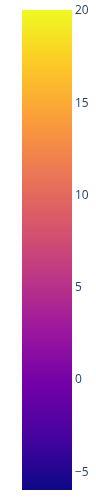
\includegraphics[height=3cm]{plots/Colorscales/Plasma.png}{Plasma}
% \caption{Colour scale for the 'Gained Points' surfaces}
% \label{fig:Plasma}
% \end{wrapfigure}
% In the following two pages, you will see all the surfaces of both Random-Discrete and Random-Continuous.
% There are five surfaces in each interaction that are generated from one ICPD.
% The x-axis, the one in be bottom-right, shows the parameter of the main strategy.
% The y-axis, the other axis on the bottom, indicates the parameter of the opponent.
% The z-axis always shows the points.
% All the surfaces are not only marked by height but also by colour.
% The context in which points are displayed depends on the surface. 
% The first two rows are the most basic surface plots.
% They show the gains of the strategy itself and the opponent's.
% The highest point that can appear is at 30.
% And the lowest is at 0.
% The maximum can be calculated by regarding the pay-off equations.
% The maximum points are gained by exploitation.
% So, $P_A =  y - c \cdot x + c$ becomes by substitution $P_A = 1 - 0.5 \cdot 0 + 0.5$ \textrightarrow $P_A = 1.5$.
% And since the CPD is played 20 times, $P_A \cdot 20 = 30$.
% So, the boundaries in which the points can vary is from 0 to 30.
% All the points, that are at height 20, have their correspondence in the other surface since in order to get 20 points, mutual cooperation is required.
% The same principle can be allied to the maximum, minimum points and mutual defection which is at height 10.
% Wherever a minimum point can be seen, the correspondence is the maximum point at the same x-y-coordinate.
% The colour of the points indicates the same as the height, the number of points.
% So, one can read this surface more accurately by regarding Figure \ref{fig:Plasma}.
% The next two surfaces concern the advantage one strategy has over the other.
% This shows us how much more one strategy had over the other.
% For the surface of the main strategy, simply the opponent's surface is subtracted from it's surface and vice versa.
% The maximum and the minimum can be calculated by taking the difference of the maximum and the minimum of the first two surfaces.
% So, the points can vary between -30 and 30.
% (30 - 0 = 30, 0 - 30 = -30)
% The two initial surfaces would intersect if they were put into one coordinate system.
% The intersection is at all the locations where the both strategies have gained an equal amount of points.
% At this location of the intersection, the surface plot, that demonstrates the advantage, would intersect with the zero-plane because the difference of two same number is always equal to zero.\\
% The two advantage surfaces are always mirrored by the zero-plane since every time you subtract $A-B$, it is the same as $(B-A) \cdot -1$.\\
% If this surface plot happens to be completely over the zero-plane, it means that the displays strategy has won every game they have played.
% Also here, there is a colour scale.
% This colour scale, however, differs from the first one.
% I chose to use different colour scales for visualisation purposes due to the fact that the advantage surfaces have a different z-axis range than the first two.
% (-30 to 30)
% B)
% % 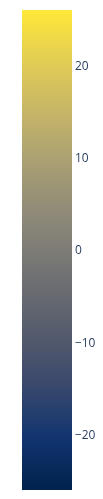
\includegraphics[height=3.0cm]{plots/Colorscales/Cividis.png}
% The last row of surfaces displays how much points have been gained by both.
% To generate these surfaces, one must add the surfaces which describe how much one has gained of the concerned strategies.
% Looking at the pay-off equations, a point can not be over the limit of 20.
% Both gain the most if both cooperate.
% Following the equations, one gets 1 point after every round.
% Since 20 rounds are played in total, the maximum is at 20.
% (20 rounds * 1 point = 20 points)
% I decided to also plot this surface to demonstrate the population welfare.
% This means that the higher the points, the most have gained both together.
% This plot has, as the advantage surfaces, a different z-axis range.
% So a new colour scale is introduced.
% C)
\newpage

% 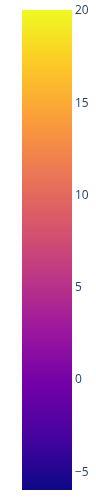
\includegraphics[height=3cm]{plots/Colorscales/Plasma.png}
% 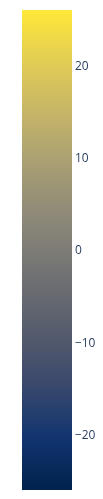
\includegraphics[height=3cm]{plots/Colorscales/Cividis.png}
% 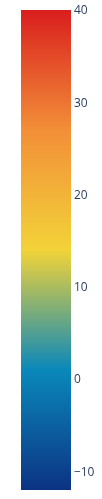
\includegraphics[height=3cm]{plots/Colorscales/Portland.png}

\newpage

\def\w{0.15}
\def\h{0.0cm}
\def\a{0}
\def\pboxb{2cm}
\def\pboxv{3.4cm}

% ------------------------------- Random-Discrete -------------------------------
\begin{figure}[!ht]
	{\sffamily
	\footnotesize
	\centering

	% Header row
	\begin{tabular}{p{0.7cm}ccccc}
		& \rotatebox{\a}{\parbox{\pboxb}{\centering Random-Discrete}} & \rotatebox{\a}{\parbox{\pboxb}{\centering Random-Continuous}} & \rotatebox{\a}{\parbox{\pboxb}{\centering Always-Same}} & \rotatebox{\a}{\parbox{\pboxb}{\centering Adapt-Discrete}} & \rotatebox{\a}{\parbox{\pboxb}{\centering Adapt-Continuous}} \\[0.2cm]

		% Gain Random-Discrete row
		\rotatebox{90}{\parbox{\pboxv}{\centering Absolute-Gain\\Random-Discrete}} &
		\includegraphics[width=\w\textwidth]{plots/Random-Discrete/Random-Discrete_vs_Random-Discrete_2/Random-Discrete.png} &
		\includegraphics[width=\w\textwidth]{plots/Random-Discrete/Random-Discrete_vs_Random-Continuous/Random-Discrete.png} &
		\includegraphics[width=\w\textwidth]{plots/Random-Discrete/Random-Discrete_vs_Always-Same/Random-Discrete.png} &
		\includegraphics[width=\w\textwidth]{plots/Random-Discrete/Random-Discrete_vs_Adapt-Discrete/Random-Discrete.png} &
		\includegraphics[width=\w\textwidth]{plots/Random-Discrete/Random-Discrete_vs_Adapt-Continuous/Random-Discrete.png} \\[\h]

		% Gain Opponent row  
		\rotatebox{90}{\parbox{\pboxv}{\centering Absolute-Gain\\Opponent}} &
		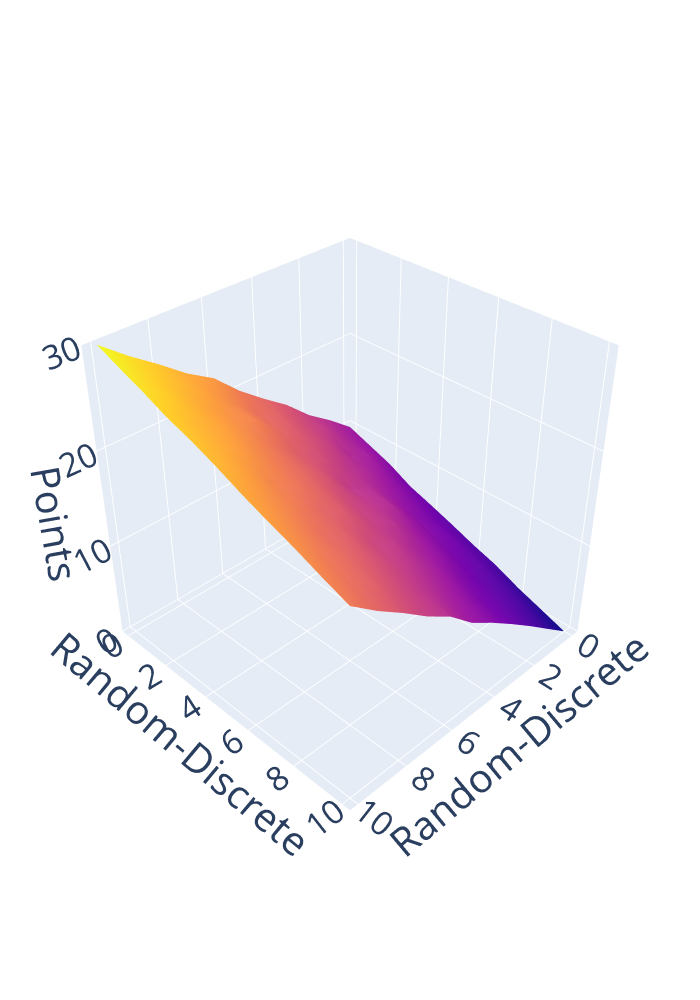
\includegraphics[width=\w\textwidth]{plots/Random-Discrete/Random-Discrete_vs_Random-Discrete_2/Random-Discrete_2.png} &
		\includegraphics[width=\w\textwidth]{plots/Random-Discrete/Random-Discrete_vs_Random-Continuous/Random-Continuous.png} &
		\includegraphics[width=\w\textwidth]{plots/Random-Discrete/Random-Discrete_vs_Always-Same/Always-Same.png} &
		\includegraphics[width=\w\textwidth]{plots/Random-Discrete/Random-Discrete_vs_Adapt-Discrete/Adapt-Discrete.png} &
		\includegraphics[width=\w\textwidth]{plots/Random-Discrete/Random-Discrete_vs_Adapt-Continuous/Adapt-Continuous.png} \\[\h]

		% Advantage Random-Discrete row
		\rotatebox{90}{\parbox{\pboxv}{\centering Relative-Gain\\Random-Discrete}} &
		\includegraphics[width=\w\textwidth]{plots/Random-Discrete/Random-Discrete_vs_Random-Discrete_2/Random-Discrete_diff.png} &
		\includegraphics[width=\w\textwidth]{plots/Random-Discrete/Random-Discrete_vs_Random-Continuous/Random-Discrete_diff.png} &
		\includegraphics[width=\w\textwidth]{plots/Random-Discrete/Random-Discrete_vs_Always-Same/Random-Discrete_diff.png} &
		\includegraphics[width=\w\textwidth]{plots/Random-Discrete/Random-Discrete_vs_Adapt-Discrete/Random-Discrete_diff.png} &
		\includegraphics[width=\w\textwidth]{plots/Random-Discrete/Random-Discrete_vs_Adapt-Continuous/Random-Discrete_diff.png} \\[\h]

		% Advantage Opponent row
		\rotatebox{90}{\parbox{\pboxv}{\centering Relative-Gain\\Opponent}} &
		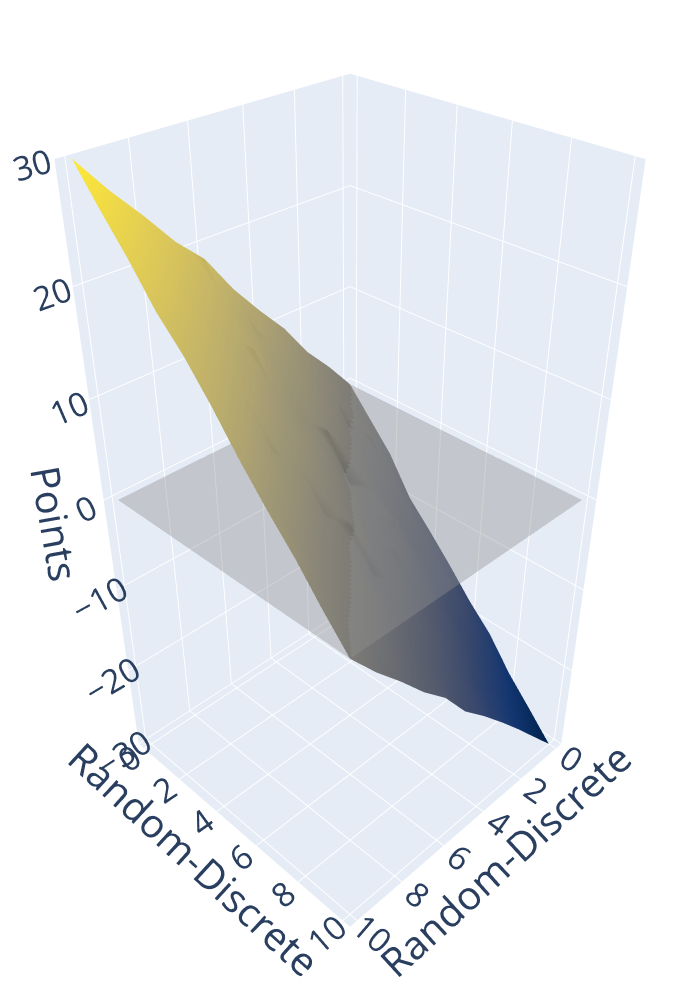
\includegraphics[width=\w\textwidth]{plots/Random-Discrete/Random-Discrete_vs_Random-Discrete_2/Random-Discrete_2_diff.png} &
		\includegraphics[width=\w\textwidth]{plots/Random-Discrete/Random-Discrete_vs_Random-Continuous/Random-Continuous_diff.png} &
		\includegraphics[width=\w\textwidth]{plots/Random-Discrete/Random-Discrete_vs_Always-Same/Always-Same_diff.png} &
		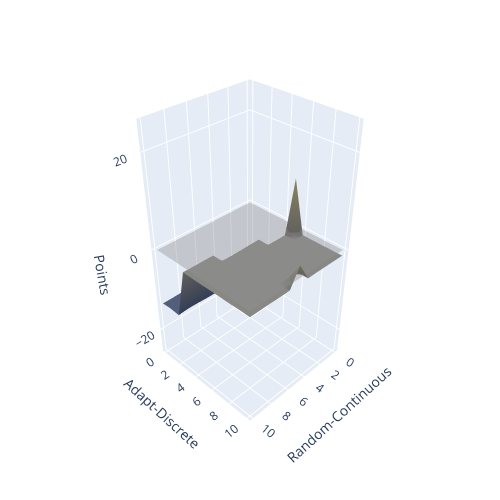
\includegraphics[width=\w\textwidth]{plots/Random-Discrete/Random-Discrete_vs_Adapt-Discrete/Adapt-Discrete_diff.png} &
		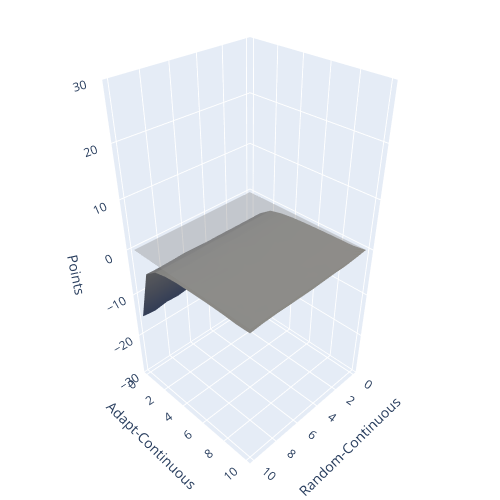
\includegraphics[width=\w\textwidth]{plots/Random-Discrete/Random-Discrete_vs_Adapt-Continuous/Adapt-Continuous_diff.png} \\[\h]

		% Overall Gain row
		\rotatebox{90}{\parbox{\pboxv}{\centering Overall-Gain\\Both Players}} &
		\includegraphics[width=\w\textwidth]{plots/Random-Discrete/Random-Discrete_vs_Random-Discrete_2/added.png} &
		\includegraphics[width=\w\textwidth]{plots/Random-Discrete/Random-Discrete_vs_Random-Continuous/added.png} &
		\includegraphics[width=\w\textwidth]{plots/Random-Discrete/Random-Discrete_vs_Always-Same/added.png} &
		\includegraphics[width=\w\textwidth]{plots/Random-Discrete/Random-Discrete_vs_Adapt-Discrete/added.png} &
		\includegraphics[width=\w\textwidth]{plots/Random-Discrete/Random-Discrete_vs_Adapt-Continuous/added.png} \\
	\end{tabular}
	\tableComp
	\caption{pbICPD surface plots for Random-Discrete. Absolute-, Relative-, and Overall-Gain values (rows) are shown for each implemented strategy (columns). Parameter value meanings for each strategy are repeated to enhance comprehensibility (Table \ref{table:strategies_overview}).}
	\label{fig:RNDD-table}
	}
\end{figure}


\newpage
% ------------------------------- Random-Continuous -------------------------------
\begin{figure}[!ht]
	{\sffamily
	\footnotesize
	\centering
    
	% Header row
	\begin{tabular}{p{0.7cm}ccccc}
		& \rotatebox{\a}{\parbox{\pboxb}{\centering Random-Discrete}} & \rotatebox{\a}{\parbox{\pboxb}{\centering Random-Continuous}} & \rotatebox{\a}{\parbox{\pboxb}{\centering Always-Same}} & \rotatebox{\a}{\parbox{\pboxb}{\centering Adapt-Discrete}} & \rotatebox{\a}{\parbox{\pboxb}{\centering Adapt-Continuous}} \\[0.2cm]
		
		% Gain Random-Continuous row
		\rotatebox{90}{\parbox{\pboxv}{\centering Absolute-Gain\\Random-Continuous}} &
		\includegraphics[width=\w\textwidth]{plots/Random-Continuous/Random-Continuous_vs_Random-Discrete/Random-Continuous.png} &
		\includegraphics[width=\w\textwidth]{plots/Random-Continuous/Random-Continuous_vs_Random-Continuous_2/Random-Continuous.png} &
		\includegraphics[width=\w\textwidth]{plots/Random-Continuous/Random-Continuous_vs_Always-Same/Random-Continuous.png} &
		\includegraphics[width=\w\textwidth]{plots/Random-Continuous/Random-Continuous_vs_Adapt-Discrete/Random-Continuous.png} &
		\includegraphics[width=\w\textwidth]{plots/Random-Continuous/Random-Continuous_vs_Adapt-Continuous/Random-Continuous.png} \\[\h]		
		% Gain Opponent row  
		\rotatebox{90}{\parbox{\pboxv}{\centering Absolute-Gain\\Opponent}} &
		\includegraphics[width=\w\textwidth]{plots/Random-Continuous/Random-Continuous_vs_Random-Discrete/Random-Discrete.png} &
		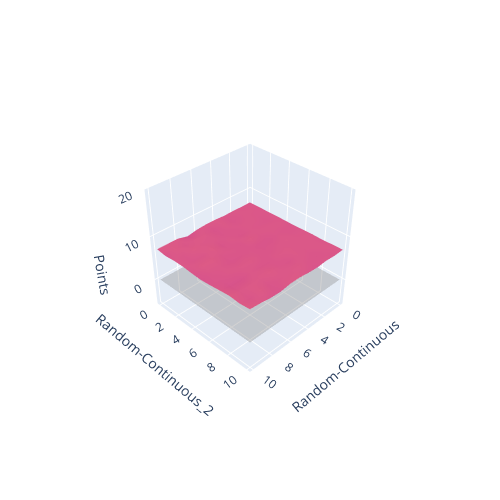
\includegraphics[width=\w\textwidth]{plots/Random-Continuous/Random-Continuous_vs_Random-Continuous_2/Random-Continuous_2.png} &
		\includegraphics[width=\w\textwidth]{plots/Random-Continuous/Random-Continuous_vs_Always-Same/Always-Same.png} &
		\includegraphics[width=\w\textwidth]{plots/Random-Continuous/Random-Continuous_vs_Adapt-Discrete/Adapt-Discrete.png} &
		\includegraphics[width=\w\textwidth]{plots/Random-Continuous/Random-Continuous_vs_Adapt-Continuous/Adapt-Continuous.png} \\[\h]		
		% Advantage Random-Continuous row
		\rotatebox{90}{\parbox{\pboxv}{\centering Relative-Gain\\Random-Continuous}} &
		\includegraphics[width=\w\textwidth]{plots/Random-Continuous/Random-Continuous_vs_Random-Discrete/Random-Continuous_diff.png} &
		\includegraphics[width=\w\textwidth]{plots/Random-Continuous/Random-Continuous_vs_Random-Continuous_2/Random-Continuous_diff.png} &
		\includegraphics[width=\w\textwidth]{plots/Random-Continuous/Random-Continuous_vs_Always-Same/Random-Continuous_diff.png} &
		\includegraphics[width=\w\textwidth]{plots/Random-Continuous/Random-Continuous_vs_Adapt-Discrete/Random-Continuous_diff.png} &
		\includegraphics[width=\w\textwidth]{plots/Random-Continuous/Random-Continuous_vs_Adapt-Continuous/Random-Continuous_diff.png} \\[\h]
		
		% Advantage Opponent row
		\rotatebox{90}{\parbox{\pboxv}{\centering Relative-Gain\\Opponent}} &
		\includegraphics[width=\w\textwidth]{plots/Random-Continuous/Random-Continuous_vs_Random-Discrete/Random-Discrete_diff.png} &
		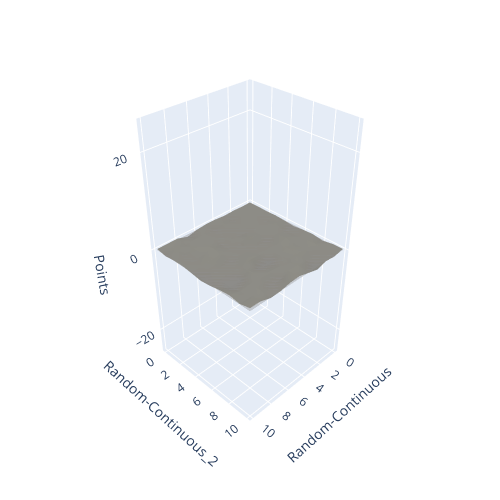
\includegraphics[width=\w\textwidth]{plots/Random-Continuous/Random-Continuous_vs_Random-Continuous_2/Random-Continuous_2_diff.png} &
		\includegraphics[width=\w\textwidth]{plots/Random-Continuous/Random-Continuous_vs_Always-Same/Always-Same_diff.png} &
		\includegraphics[width=\w\textwidth]{plots/Random-Continuous/Random-Continuous_vs_Adapt-Discrete/Adapt-Discrete_diff.png} &
		\includegraphics[width=\w\textwidth]{plots/Random-Continuous/Random-Continuous_vs_Adapt-Continuous/Adapt-Continuous_diff.png} \\[\h]		
		% Overall Gain row
		\rotatebox{90}{\parbox{\pboxv}{\centering Overall-Gain\\Both Players}} &
		\includegraphics[width=\w\textwidth]{plots/Random-Continuous/Random-Continuous_vs_Random-Discrete/added.png} &
		\includegraphics[width=\w\textwidth]{plots/Random-Continuous/Random-Continuous_vs_Random-Continuous_2/added.png} &
		\includegraphics[width=\w\textwidth]{plots/Random-Continuous/Random-Continuous_vs_Always-Same/added.png} &
		\includegraphics[width=\w\textwidth]{plots/Random-Continuous/Random-Continuous_vs_Adapt-Discrete/added.png} &
		\includegraphics[width=\w\textwidth]{plots/Random-Continuous/Random-Continuous_vs_Adapt-Continuous/added.png} \\
	\end{tabular}
	\tableComp
	\caption{pbICPD surface plots for Random-Continuous. Absolute-, Relative-, and Overall-Gain values (rows) are shown for each implemented strategy (columns). Parameter value meanings for each strategy are repeated to enhance comprehensibility (Table \ref{table:strategies_overview}).}
	\label{fig:RNDC-table}
	}
\end{figure}


\newpage

\noindent
In the following two subsections (\ref{sec:desc_RD}, \ref{sec:desc_RC}), the results of each column of each figure, meaning the five surface plots, will be described.
The description follows a certain patter: First, the two absolute-gain, second, both relative-gain, and third, the overall-gain surfaces are explained in more detail.

\subsection{Random-Discrete} \label{sec:desc_RD}

\subsubsection*{Random-Discrete}
		The left (10, 0) and right (0, 10) corner are the extremes of the surface.
		Random-Discrete is exploited if its parameter equals 10, meaning it corresponds to AlwaysCooperate, and the parameter of Random-Discrete as an opponent is 0, i.e., equivalent to AlwaysDefect.
		% This is how one can get the maximum output, by exploiting.
		% This can be seen in the surface of Random-Discrete\textunderscore2.
		The rearmost corner at the coordinate (0, 0) is where both players defect constantly, which relates to the already clarified fact that this point is located at a height of 10 for both players.
		% This is the point where both get their relative lowest output, as can be seen later.\\
		When both parameters equal 10, both points have a z-component of 20.
		This indicates that both strategies behave equally, i.e., as AlwaysCooperate, which leads to a gain of 20 points separately.

		The peaks of both relative-gain surfaces derive from the maximum outputs of the pay-off system.
		Since one can get the maximum output only if the other is exploited, the relative-gain surfaces entail the extreme outcomes of the ICPD.
		When the two parameters are identical, however, no strategy wins.

		The overall-gain surface clearly indicates that the peak of the surface is at (10, 10).
		This point has the quality that both strategies are equivalent to AlwaysCooperate.
		% This illustrates the dilemma pretty well.
		The rearmost point, being the lowest, results from the fact that both defected constantly.
		So, for the welfare of the population, it is best if both always cooperate.
		In sum, this is the standard outcome of the PD game.

\subsubsection*{Random-Continuous}
		The absolute-gain surfaces concerning the interaction of Random-Discrete and Random-Continuous continuously range from 20 to 10 and from 5 to 25, respectively.
		Both surfaces are not influenced by the parameter of Random-Continuous.

		% This is logical and will be looked at the discussion.\\

		The two relative-gain surfaces, show that Random-Discrete wins if the parameter values are lower than 5, which corresponds to defecting with a higher probability than 50\%.
		For the parameter values higher than 5, i.e., cooperating more than defecting, the contrary is true.
		The relative-gain surfaces range continuously from -15 to 15.

		The overall-gain surface shows a constant slope with points ranging from 35 to 25.
		The maximum value of 40 is not achieved since full exploitation does not take place.
		The fact that the surfaces are not affected by the parameter value of Random-Continuous will be analysed in the discussion section \ref{sec:discussion}.

\subsubsection*{Always-Same}
		Remarkably, Always-Same behaves exactly like Random-Discrete.
		This becomes visible when looking at the columns where Random-Discrete plays against itself and against Always-Same.
		The surprising absence of any difference between these two strategies needs further explanation and will thus be revisited in the discussion section \ref{sec:discussion}.

\subsubsection*{Adapt-Discrete}
		In the absolute-gain surface of Random-Discrete against Adapt-Discrete, a stripe appears at Adapt-Discrete parameter values from 0 to 2.
		This stripe ranges from absolute exploitation at (0, 0) to mutual cooperation where the parameter of Random-Discrete is equal to 10.
		Abruptly, this stripe does not continue to follow its pattern in the y-direction, rather a new inclination is visible.
		Both surfaces' lowest points are at a height of 10, which means that---after adaptation of Adapt-Discrete---mutual defection was played.
		However, if Random-Discrete always cooperates, the same effect appears, due to the adaptation of Adapt-Discrete, mutual cooperation can be observed resulting in 20 points for both players. 
		Additionally, the maximum points of the first plot indicate that the same points on the corresponding surface of the opponent must be at height 0.
		% The broader slope is also going downwards.
		% But this slope is not as steep as the one on the other surface and thus has lower points at the edge where the parameter of Random-Discrete is 0.
		% When Random-Discrete has its parameter at 10, which means it behaves like AlwaysCooperate, mutual cooperation will take place.\\

		The relative-gain surfaces---with the exception of the stripe highlighted above---is close to 0, meaning that there are practically no advantages.
		At the coordinates of the stripe, however, a remarkable advantage for Random-Discrete over Adapt-Discrete stands out, which needs further discussion (\ref{sec:discussion}).

		As a matter of course, the overall-gain surface shows highest points where only mutual cooperation occurs, which is where the parameter of Random-Discrete is equal to 10 and Adapt-Discrete adapts to this value.
		The rear end of the stripe is at a height of 30 which indicates full exploitation.
		And the broader subsurface ends at a height of 20 which suggests mutual defection.
		Once again, the reason for this discontinuity will be analysed in the discussion (\ref{sec:discussion}). 

\subsubsection*{Adapt-Continuous}
		The absolute-gain surfaces considerably resemble the ones of the Adapt-Discrete interaction.
		The difference mainly concerns the angularity since curves appear to replace the edges.
		So on the one hand, the similarity can be attributed to the description already delivered for Adapt-Discrete.
		On the other hand, the rounding off effect needs further investigation in the discussion (\ref{sec:discussion}).
		% The edge where points are at height 20, stays as it was in the game against Adapt-Discrete.
		% The broad slope is also similar to that surface, its lowest points being at 10.
		% The surface of Adapt-Continuous is in a same way similar to the one of Adapt-Discrete.
		% The edges are curved out.
		% But, the slope is, again, a bit steeper than the one of Random-Discrete.\\
		The same applies to the relative-gain and overall-gain surface plots.\\

		% The advantage surface of Adapt-Continuous is in a difficult angle to see.
		% The origin of the coordinate-system is the lowest point of this surface.
		% I concluded this fact by knowing that the highest point of the other advantage surface has its correspondence at height 0.\\
		%
		% The maximum points are aligned in a line.
		% More specific, an edge of the surface at height 40.
		% The least points are gained at the edge more behind at the y-z-plane.
		% This edge is rather a curve than a straight line.
		% This curve bows from exploitation at coordinates being at (0, 0) to 20, the absolute minimum of this surface.
	
\subsection{Random-Continuous} \label{sec:desc_RC}

\subsubsection*{Random-Discrete}
	The interaction of Random-Discrete and Random-Continuous has already been described above (\ref{sec:desc_RD}).
	So, no further explanation is required.

\subsubsection*{Random-Continuous}
	The interaction of Random-Continuous with itself results in completely flat surfaces.
	The absolute-gain surfaces are at a height of 15.
	This can be ascribed to the fact that Random-Continuous on average delivers 0.5 as an investment.
	% We can calculate at which height the surface is.
	Plugging in 0.5 for both $x$ and $y$ in the pay-off equations (see \ref{sec:iterated_continuous_prisoners_dilemma}), we get $p_A = p_B = 0.5 - 0.5 \cdot 0.5 + 0.5$ \textrightarrow $p_A = p_B = 0.75$.
	After 20 rounds of the CPD, this comes down to 15 points for both players.

	Subtracting two flat surfaces at the same height results in an also flat surface which corresponds to the zero-plane.
	No strategy was better than the other at any point.

	Adding these two even surfaces---which are both at height 15---an overall surface at height 30 follows.
	The flatness of all the surfaces deserves to be revisited in the discussion (\ref{sec:discussion}).

\subsubsection*{Always-Same}
	As already observed in the subsection on the Random-Discrete strategy (\ref{sec:desc_RD}), Always-Same behaves identically to Random-Discrete.
	Once again, this effect requires further examination in the discussion section (\ref{sec:discussion}).

\subsubsection*{Adapt-Discrete}
	For the absolute-gain plots, there are two main levels of the surfaces.
	The upper level in the Random-Continuous surface is at a height of 25 and the lower one at a height of 10.
	Additionally, there is a little peak at the coordinate (5, 10) with an approximate height of 17 and 12, respectively.
	The lower level in the Adapt-Discrete surface is located at a height of 10 and the upper one at a height of 15 while the peak is pointing downwards.

	The upper level of the absolute-gain surface of Random-Continuous is approximately 15 points higher than the lower level of the other absolute-gain plot.
	Additionally, the lower level of the surface of Random-Continuous and the upper one of the surface of Adapt-Discrete have almost the same z value.
	Notably, the relative-gain surface of Random-Continuous is completely above the zero-plane, which pronouncedly applies for small parameter values of Adapt-Discrete, i.e., corresponding to AlwaysCooperate.
	This means that Random-Continuous won the entire pbICPD.

	In terms of overall-gain, the upper level of the absolute-gain surface of Random-Continuous added to the lower level of the one of Adapt-Discrete results in higher values than adding the two levels of similar height.
	Furthermore, a small positive peak remains.
	Again, the reason for this discontinuity will be discussed later (\ref{sec:discussion}).

\subsubsection*{Adapt-Continuous}
	The absolute-gain surfaces resemble a wave or a curve in the y-direction.
	The fact that the Random-Continuous parameter does not affect the surface's form can be traced back to the already discussed phenomenon that Random-Continuous on average behaves like AlwaysNeutral.
	Strikingly, the upper and lower limits of the surfaces correspond to the absolute-gain surfaces described above for the Adapt-Discrete interaction.
	For Adapt-Continuous parameter values of higher than three, the curved surface appears to pronouncedly converge to a flat plane at a height of about 15.

	The same properties can be seen in the relative-gain surface plots.
	Upper and lower limits correspond to those of the relative-gain surfaces of the Adapt-Discrete interaction and the relative-gain surface of Random-Continuous is again completely located above the zero-plane.
	The same applies to the overall-gain surface plot with its upper limit at a height of 35 and the lower limit at a height of 30.
	The reasons for this curvature will be revisited in the discussion (\ref{sec:discussion}).


\section{Discussion} \label{sec:discussion}

% The results suggest certain effects of the PD.
In the results section (\ref{sec:results}), several issues have been identified that deserve a closer inspection.
In the following subsections, these issues will be discussed in regard to aspects of shallow randomness (\ref{sec:shallow_randomness}), dispersion and risk (\ref{sec:dispersion_risk}), threshold values for discrete adaptations (\ref{sec:threshold_values}), and dynamics of continuous adaptations (\ref{sec:dynamics}).
Finally, the interactions in terms of gains against random strategies will be referred back to the leading question of the present thesis (\ref{sec:conclusion_discuss}).

\subsection{Shallow Randomness} \label{sec:shallow_randomness}

	It was found that Random-Discrete acts identically as Always-Same and Random-Continuous as AlwaysNeutral.
	This means that Random-Discrete and Random-Continuous, as random strategies, behave equitably as deterministic strategies if the average of all the generated surfaces is taken.
	% The mathematical framework used to describe this phenomenon is called the Law of Large Numbers (LLN).
		
	To clarify the resemblance between Random-Discrete and Always-Same, the equations to calculate the investment have to be analysed (see Equation \ref{eq:RD_i_eq_1}).


	\begin{equation}
		\Pr(i = 1) = \frac{1}{10} \theta_{\mathrm{RD}}
		\label{eq:RD_i_eq_discuss}
	\end{equation}

	% \begin{equation}
	% 	\begin{split}
	% 	% \Pr(i = 1 \mid \theta_{\mathrm{RndD}}) = \frac{\theta_{\mathrm{RndD}}}{10}
	% 	% \text{ or }
	% 	% i \;\sim\; \mathrm{Bernoulli}(\frac{\theta_{\mathrm{RndD}}}{10})\\
	% 	i \;\sim\;
	% 	\begin{cases}
	% 	  1 & \text{with probability } \frac{1}{2}\\
	% 	 -1 & \text{with probability } \frac{1}{2} 
	% 	\end{cases}
	% 	\label{eq:RNDD_i_eq}
	% 	\end{split}
	% \end{equation}

	\noindent
	Regarding the investment calculation of Random-Discrete (Equation \ref{eq:RD_i_eq_discuss}), we can generate $n$ investments (Equation \ref{eq:RD_n_i}).

	\begin{equation}
		% \epsilon_1, \epsilon_2, \epsilon_3, \dots, \epsilon_n \;\sim 2 \cdot \mathrm{Bernoulli}(\frac{1}{2}) - 1
		i_1, i_2, i_3, \dots, i_n = 
		\begin{cases}
		1 & \text{with probability } \frac{1}{10} \theta_{\mathrm{RD}}\\
		0 & \text{with probability } 1 - \frac{1}{10} \theta_{\mathrm{RD}} 
		\end{cases}
		\label{eq:RD_n_i}
	\end{equation}

	\noindent
	The average of all the generated investments in Equation \ref{eq:RD_n_i} converges to a certain value as shown in Equation \ref{eq:RD_i_avr}.

	\begin{equation}
		\bar i = \lim_{n\to\infty} \frac{1}{n} \sum_{k=1}^{n} i_k = \theta_{\mathrm{RD}} \frac{1}{10} \text{ almost surely}
	\label{eq:RD_i_avr}
	\end{equation}

	\noindent
	Substituting $n$ with 100---the number of repetitions in the present simulation---in Equation \ref{eq:RD_i_avr} would be an approximation.
	% But, for the scope of this project, 100 repetitions were chosen to be sufficient.

	\begin{equation}
		\bar i \approx \frac{1}{100} \sum_{k=1}^{100} i_k \approx \theta_{\mathrm{RD}} \frac{1}{10}
		\label{eq:RD_approx_i}
	\end{equation}

	\noindent
	Hence, calculating an investment with a certain probability ultimately comes down to investing the same contribution constantly, which in turn corresponds to the behaviour of Always-Same.\\

	\noindent
	A similar effect applies for Random-Continuous and the convergence to the behaviour of the AlwaysNeutral strategy.
	To investigate this effect, the same procedure is conducted.
	First, the investment equations of Random-Continuous need to be revisited (see Equations \ref{eq:RC_i_eq}-\ref{eq:RC_e_prob}).

	\begin{equation}
		i(\theta_{\mathrm{RC}}) = 0.5 + \epsilon \cdot s(\theta_{\mathrm{RC}})
		\label{eq:}
	\end{equation}
	\begin{equation}
		s(\theta_{\mathrm{RC}}) = \theta_{\mathrm{RC}} \frac{1}{20}
		\label{eq:}
	\end{equation}
	\begin{equation}
		\begin{split}
		% \Pr(\epsilon = 1) = \Pr(\epsilon = -1) = \frac{1}{2} \text{ or } \epsilon \;\sim 2 \cdot \mathrm{Bernoulli}(\frac{1}{2}) - 1\\
		\epsilon = 
		\begin{cases}
		  1 & \text{with probability } \frac{1}{2}\\
		 -1 & \text{with probability } \frac{1}{2} 
		\end{cases}
		\label{eq:prob_eps}
		\end{split}
	\end{equation}

	\noindent
	Only Equation \ref{eq:prob_eps} contains a probability
	We thus form $n$ $\epsilon$ values, as Equation \ref{eq:RC_n_e} implies.

	\begin{equation}
		\epsilon_1, \epsilon_2, \epsilon_3, \dots, \epsilon_n = 
		\begin{cases}
		  1 & \text{with probability } \frac{1}{2}\\
		 -1 & \text{with probability } \frac{1}{2} 
		\end{cases}
		\label{eq:RC_n_e}
	\end{equation}

	\noindent	
	The average of these $\epsilon$ values cancels out and therefore equals 0 (Equations \ref{eq:RC_e_avr} and \ref{eq:RC_approx_eq}).

	\begin{equation}
		\bar \epsilon = \lim_{n\to\infty} \frac{1}{n} \sum_{k=1}^{n} \epsilon_k = 0 \text{ almost surely}\\
		\label{eq:RC_e_avr}
	\end{equation}
	\begin{equation}
		\bar \epsilon \approx \frac{1}{100} \sum_{k=1}^{100} \epsilon_k \approx 0
		\label{eq:RC_approx_eq}
	\end{equation}

	\noindent
	Consequently, the investment is---over 100 repetitions---approximately equal to 0.5, as shows Equation \ref{eq:i_eq_0.5}.

	\begin{equation}
		i(\theta_{\mathrm{RC}}) \approx 0.5 + \bar \epsilon \cdot \theta_{\mathrm{RC}} \frac{1}{20} \approx 0.5
		\label{eq:i_eq_0.5}
	\end{equation}

	\noindent
	The generally non-existent influence of Random-Continuous' parameter values can be traced back to this phenomenon---which is labelled as the Law of Large Number in mathematical statistics.


\subsection{Dispersion and Risk} \label{sec:dispersion_risk}
	
	Building on the discussions on shallow randomness (section \ref{sec:shallow_randomness}), it seems worthwhile to delve deeper into the dispersion of the Random-Discrete and Always-Same surfaces, which on average show the same behaviour.
	To this end, Figure \ref{fig:two_one-iter} illustrates the absolute-gain surfaces of the interaction of both strategies if only played once (with 20 rounds).

	\begin{figure}[h]
		\centering
		\includegraphics[width=0.45\textwidth]{plots/Discussion/Random-Discrete_vs_Always-Same/Random-Discrete_first.png}
		\includegraphics[width=0.45\textwidth]{plots/Discussion/Random-Discrete_vs_Always-Same/Always-Same_first.png}\\
		\caption{pbICPD surfaces without repetitions. Absolute-gain surfaces for Random-Discrete (left) and for Always-Same (right).}
		\label{fig:two_one-iter}
	\end{figure}

	\noindent
	Coarser surfaces are visible, which is due to the phenomenon of the Law of Large Numbers as explained above (section \ref{sec:shallow_randomness}).
	The surface of Random-Discrete is a bit evener. 
	This fact can be explained by examining the pay-off Equations \ref{eq:payoff_A} and \ref{eq:payoff_B}:
	$p_A = y - c x + c$ and $p_B = x - c y + c$, where $x$ is the previous investment of Random-Discrete and $y$ the previous investment of Always-Same.
	Since $x$ is random---depending on Random-Discrete's parameter---and $y$ is a constant over one ICPD, subtracting only a fraction of the random investment pays off a more constant amount of points.

	To calculate the dispersion of the average absolute-gain surface, the Standard Deviation (SD) (Equation \ref{eq:standard_deviation}) can be used for every game and thus new surface plots can be generated (see Figure \ref{fig:two_one-iter_sd}). 

	\begin{equation}
		s = \sqrt{\frac{1}{N-1} \sum_{i=1}^N (x_i - \overline{x})^2}
		\label{eq:standard_deviation}
	\end{equation}

	\begin{figure}[htbp]
		\centering
		\includegraphics[width=0.42\textwidth]{plots/Discussion/Random-Discrete_vs_Always-Same/Random-Discrete_sd.png}
		\includegraphics[width=0.42\textwidth]{plots/Discussion/Random-Discrete_vs_Always-Same/Always-Same_sd.png}
		\caption{pbICPD Standard-Deviation surfaces for 100 repetitions. Standard deviations of the absolute-gain surfaces of Random-Discrete (left) and of Always-Same (right).}
		\label{fig:two_one-iter_sd}
	\end{figure}

	\noindent
	As can be seen in Figure \ref{fig:two_one-iter_sd}, the SD surface of Random-Discrete is considerably smaller than that of Always-Same, which refers to the explanation already provided above.
	Furthermore, it becomes obvious that both SD surfaces are only affected by the parameter value of Random-Discrete with the highest SDs located at a parameter value of 5, which represents the most random version of the strategy. 
	To conclude, on the one hand, there is a more pronounced chance for Always-Same to win or lose if the parameter of Random-Discrete takes medium values.
	On the other hand, as can be seen in Figure \ref{fig:SD_avr}, the resulting risk is largely negligible since the average absolute-gain surfaces are not remarkably altered by the SD (which covers 68.2\% of the samples).

	\begin{figure}[h]
		\centering
		\includegraphics[width=0.45\textwidth]{plots/Discussion/Random-Discrete_vs_Always-Same/Random-Discrete_sd_p_avr.png}
		\includegraphics[width=0.45\textwidth]{plots/Discussion/Random-Discrete_vs_Always-Same/Always-Same_sd_p_avr.png}
		\caption{pbICPD surfaces after 100 repetitions. Absolute-gain surfaces $\pm$ SD for Random-Discrete (left) and for Always-Same (right).}
		\label{fig:SD_avr}
	\end{figure}

\subsection{Threshold Values for Discrete Adaptations} \label{sec:threshold_values}
		
	Regarding the surfaces of the interactions of Random-Discrete with Adapt-Discrete, a surprising stripe can be observed.
	To understand the reason for this effect, the investment calculations of Adapt-Discrete should be recalled (see Equations \ref{eq:AD_i0}-\ref{eq:AD_s_eq}).
	\begin{equation}
		i_0 = 1
		\label{eq:AD_i0_discuss}
	\end{equation}
	\begin{equation}
		i(\theta_{\mathrm{AD}}, k) =
		\begin{cases}
			1 & \text{ if } i_1 + s(\theta_{\mathrm{AD}}, k) \ge 0.5\\
			0 & \text{ if } i_1 + s(\theta_{\mathrm{AD}}, k) < 0.5\\
		\end{cases}
		\label{eq:AD_rounded}
	\end{equation}

% $$i(\theta_{\mathrm{AD}}) = \round{i_1 + s(\theta_{\mathrm{AD}})}$$
	\begin{equation}
		s(\theta_{\mathrm{AD}}, k) = \frac{1}{5} \theta_{\mathrm{AD}} \cdot (\tilde{i}_{k-1} - i_{k-1})
		\label{eq:AD_eq_s_discuss}
	\end{equation}

	\noindent
	As the investments of Adapt-Discrete are rounded to the nearest integer (Equation \ref{eq:AD_rounded}), to get from investment 0 to 1 or vice versa, the raw value of the investment has to exceed a certain threshold value which is equal to 0.5.
	In the first round, Adapt-Discrete contributes full cooperation (Equation \ref{eq:AD_i0_discuss}), so that to surpass the threshold, the shift in Equation \ref{eq:AD_eq_s_discuss} must be lower than -0.5.
	To generate a general formula that calculates the opponent's investment that is necessary to exceed the threshold in the first round given the Adapt-Discrete parameter, it is required to solve for $\tilde{i}_1$.

	\begin{equation}
\begin{alignedat}{2}
s(\theta_{\mathrm{AD}}, k)                           &< -0.5
  &\qquad& \\[5pt]
\frac{\theta_{\mathrm{AD}}}{5}(\tilde{i}_{k-1}-1)    &< -0.5
  &\qquad& \bigl|\cdot\frac{5}{\theta_{\mathrm{AD}}}\bigr.\\[5pt]
\tilde{i}_{k-1} - 1                                  &< -\dfrac{2.5}{\theta_{\mathrm{AD}}}
  &\qquad& \bigl|+1\bigr.\\[5pt]
\tilde{i}_{k-1}                                      &< -\dfrac{2.5}{\theta_{\mathrm{AD}}}+1
  &\qquad&
\end{alignedat}
\label{eq:adpd_inequality}
\end{equation}\\

	\noindent
	Figure \ref{fig:surpass_theshold_abs} illustrates this formula graphically.
	The curve depicts the upper limit of the area of values for which adaptation takes place (exclusively).
	It can be seen that the opponent's investment would be needed to fall below 0 to exceed the threshold value if $0 \le \theta_{\mathrm{AD}} \le 2$.
	However, a contribution below 0 is impossible.
	To conclude, if Adapt-Discrete's parameter is either 0, 1, or 2, the shift required to surpass the threshold value cannot be achieved.
	Thus, Adapt-Discrete is equivalent to AlwaysCooperate in cases where its parameter is lower than 3.
	This explains the gainfulness of the stripe in the absolute-gain surface of Random-Discrete and thus the corresponding disadvantage of Adapt-Discrete.
	In this area of the surface, Adapt-Discrete is exploited since it cannot react because of always submitting full cooperation.

	\begin{figure}[h]
		\begin{center}
			\includegraphics[width=0.8\textwidth]{plots/Discussion/Adapt-Discrete/Adapt-Discrete_values_surpass_threshold_abs.png}
		\end{center}
		\caption{Threshold values for discrete adaptations as a function of the Adapt-Discrete parameter.}
		\label{fig:surpass_theshold_abs}
	\end{figure}

	% Coming to the next attribute of this plot; the evenness of the rest of the surface.
	% The other part of the surface is first, not influenced by the parameter of Adapt-Discrete and second, has a little inclination.
	% The first point can be answered with the already proven fact that Random-Discrete parallels Always-Same.
	% Adapt-Discrete mimics the opposing strategy if it belongs to the rigid category since the shift is equal to zero after the first few round, as will be discussed later.% explanation needed??
	% \\
	% The second quality can be justified by becoming clear about the fact that Random-Discrete will range its contributions from 0 to 1 as its parameter increases.
	% But, a little detail can be observed concerning the inclinations of the two areas which do not coincide with each other.
	% The subarea of the absolute-gain surface of Adapt-Discrete is a smidgen steeper than the other.
	% This item substantiated by reason.
	% Adapt-Discrete's first investment is always full cooperation.
	% Random-Discrete with its parameter set to 0 acts like AlwaysDefect.
	% Adapt-Discrete is thus completely exploited in the first round.
	% Random-Discrete's parameter equal to 10, in contrary, will let Random-Discrete act like AlwaysCooperate.
	% Hence, Adapt-Discrete is not at all exploited in the first round, and will never be during the game.
	% To deduce, the nearer Random-Discrete's parameter is to zero, the more Adapt-Discrete is exploited in the first round.
	% As a consequence of that, Adapt-Discrete will have a minor point deficit at most of the games.


	\noindent
	In the surface plot of the interaction of Random-Continuous with Adapt-Discrete, the existence of two different levels is remarkable and will thus be investigated.
	% \begin{figure}
	% 	\begin{center}
	% 		\includegraphics[width=0.5\textwidth]{plots/Discussion/Random-Continuous_vs_Adapt-Discrete/surface_2D.png}
	% 	\end{center}
	% 	\caption{}
	% 	\label{fig:AdpD_2D_surface}
	% \end{figure}
	To understand the discontinuity of the two absolute-gain surfaces, the investment calculations of Random-Continuous (Equation \ref{eq:RC_i_eq}-\ref{eq:RC_e_prob}) need to be revisited.

\begin{equation}
	i(\theta_{\mathrm{RC}}) = 0.5 + \epsilon \cdot s(\theta_{\mathrm{RC}})
	\label{eq:RC_i_eq_discuss}
\end{equation}
\begin{equation}
	s(\theta_{\mathrm{RC}}) = \frac{1}{20} {\theta_{\mathrm{RC}}}
	\label{eq:RC_s_eq_discuss}
\end{equation}
\begin{equation}
	\Pr(\epsilon = 1) = \Pr(\epsilon = -1) = \frac{1}{2}
	\label{eq:RC_e_prob_discuss}
\end{equation}

	\noindent
	The investment of Random-Continuous as a function of its parameter can be found as a graph in Figure \ref{fig:RC_investm} (left).
	The lower and upper points of one parameter value are notated as 'RC [parameter value] lower' or  'RC [parameter value] upper', respectively.

	\begin{figure}[h]
		\centering
		\includegraphics[width=0.45\textwidth]{plots/Discussion/Random-Continuous/investments.png}
		\includegraphics[width=0.45\textwidth]{plots/Discussion/Random-Continuous_vs_Adapt-Discrete/Adapt-Discrete_values_surpass_threshold_abs.png}
		\caption{Investment of Random-Continuous as a function of its parameter (left) and intersections of parameter-dependent investments with the \emph{'Threshold values'} from Figure \ref{fig:surpass_theshold_abs} (right).}
		\label{fig:RC_investm}
	\end{figure}

	\noindent
	As shown in Figure \ref{fig:RC_investm} (right), every investment of Random-Continuous above the line of \textit{'Threshold Values'} results in an exploitation of Adapt-Discrete.
	Parameters equal to either 0, 1, or 2 necessitate a different approach (as discussed above).
	To explain this fact, the parameter value of Adapt-Discrete equal to 3 will be taken as an example.
	The same idea applies to every further value of the parameter.
	The graph at parameter 3 is at an investment value of $0.1\overline{6}$ and thus lies between the lines \textit{'RC 7 Lower'} and \textit{'RC 6 Lower'}.
	The line below this point means that this and every greater parameter of Random-Continuous does not exploit Adapt-Discrete.
	% Adapt-Discrete can surpass the threshold value of 0.5 because the investment of Random-Continuous 7 and every further one submits a lower investment (with a 50\% change) and thus defects completely.
	The line above indicates the first version of Random-Continuous in negative direction that exploits Adapt-Discrete.
	This line can be at the same height as the point and it would still result in a losing situation for Adapt-Discrete.\\
	
	\noindent 
	The appearance of the small peak is also a part of the discontinuity of the surfaces.
	In Figure \ref{fig:RndC_AdpD_peak} it can be seen that the two traces \textit{'RC 5 Lower'} and \textit{'RC 5 Upper'} intersect with \textit{'Surpass Threshold Down'} and \textit{'Surpass threshold Up'} where the parameter value of Adapt-Discrete is equal to 10, respectively.
	In the first round---as Adapt-Discrete starts with full cooperation---Adapt-Discrete only adapts from 1 to 0 with a probability of 50\% since only the investment line \textit{'RC 5 lower'} is located below the point of the \textit{'Surpass threshold down'} curve.
	However, Adapt-Discrete always surpasses the threshold value of 0.5 from full defection to full cooperation as both \textit{'RC 5 Lower'} and \textit{'RC 5 Upper'} are above the corresponding point of the \textit{'Surpass Threshold Up'} graph.
	Therefore, Adapt-Discrete will go down in 50\% of the cases when it is at full cooperation but it will go up to full cooperation when it is at full defection with 100\% probability.
	This implies that Adapt-Discrete is exploited more often because Adapt-Discrete cooperates more often than it defects.
	Every other combination of parameters of Adapt-Discrete and Random-Continuous prevents this situation from occurring.


	% The reason for the existence of the peak at coordinates $(5, 10, z)$ has not yet been clarified.
	\begin{figure}[h]
		\centering
		\includegraphics[width=0.5\textwidth]{plots/Discussion/Random-Continuous_vs_Adapt-Discrete/Adapt-Discrete_values_surpass_threshold_up.png}
		\caption{Intersections of surpass thresholds curves with \emph{'RC 5 Lower'} and \emph{'RC 5 Upper'}.}
		\label{fig:RndC_AdpD_peak}
	\end{figure}
	% Figure \ref{fig:RndC_AdpD_peak} demonstrate this aspect.


\subsection{Dynamics of Continuous Adaptations} \label{sec:dynamics}
	
	The absolute-gain surface of Adapt-Continuous in the interaction with Random-Discrete has similar qualities to that of Adapt-Discrete against Random-Discrete.
	The main difference between these surfaces concerns the angularity.
	% A same idea can be used to explain the similar appearance of the surfaces against Adapt-Continuous compared to the ones against Adapt-Discrete.
	Figure \ref{fig:AC_approx_invetm_and_payoffs_0-5} demonstrates the investments of Adapt-Continuous in one ICPD when it plays against Random-Discrete, thereby taking Always-Same as equivalent to Random-Discrete for simplicity (see \ref{sec:shallow_randomness} and \ref{sec:dispersion_risk}).
	Adapt-Continuous pursuits getting on the same level of investment as the opponent for parameter values from 1 to 5.
	Parameter 0 forms a special case as its strategy never adapts and thus always cooperates, which can be derived from the fact that the difference to the opponent's investment is multiplied by 0 and thus no adaption is made.
	The parameter value of Random-Discrete equals 5 in Figure \ref{fig:AC_approx_invetm_and_payoffs_0-5}.

	% Always-Same vs Adapt-Continuous better?
	\begin{figure}[h!]
		\centering
		\includegraphics[width=0.45\textwidth]{plots/Discussion/Adapt-Continuous/Approx_5_line_chart_0-5.png}
		\includegraphics[width=0.45\textwidth]{plots/Discussion/Adapt-Continuous/Approx_pay-offs_5_line_chart_0-5.png}
		\caption{Investments (left) and pay-offs (right) of Adapt-Continuous with parameters ranging from 0 to 5 against Random-Discrete parameter 5 as a functions of the iteration.}
		\label{fig:AC_approx_invetm_and_payoffs_0-5}
	\end{figure}
	
	\noindent
	In Figure \ref{fig:AC_approx_invetm_and_payoffs_0-5} (left), the mathematical function for each graph can be derived from the investment calculation of Adapt-Continuous (Equations \ref{eq:AC_i0}-\ref{eq:AC_s_eq}).
	Equation \ref{eq:AdpC_i_eq_rec} describes this process recursively.
	$k$ indicates the current round and $\theta$ is the parameter of Adapt-Continuous.
	$\tilde{i}$ is the opponent's investment and thus constant.
	\begin{equation}
		i_k = i_{k-1} + \frac{1}{5}\theta \cdot (\tilde{i} - i_{k-1})
		\label{eq:AdpC_i_eq_rec}
	\end{equation}

	\noindent
	% derivation in appendix (ChatGPT)
	Since it is not possible to generate a graph using the recursive form, the explicit version is required (Equation \ref{eq:AdpC_i_eq_expl}).

	\begin{equation}
		i_k = \tilde{i} + (1 - \frac{1}{5}\theta)^k \cdot (i_0 - \tilde{i})
		\label{eq:AdpC_i_eq_expl}
	\end{equation}
	
	\noindent
	The higher the parameter of Adapt-Continuous, the faster the strategy can adjust its investment.
	This means that Adapt-Continuous, when the parameter is small, will be more exploited in the first several rounds than an Adapt-Continuous version with a larger parameter value.
	For parameter values of Adapt-Continuous greater than or equal to 5, Figure \ref{fig:AC_approx_invetm_and_payoffs_5-10} shows the dynamics of the investments and pay-offs.

	\begin{figure}[!h]
		\centering
		\includegraphics[width=0.49\textwidth]{plots/Discussion/Adapt-Continuous/Approx_5_line_chart_5-10.png}
		\includegraphics[width=0.49\textwidth]{plots/Discussion/Adapt-Continuous/Approx_pay-offs_5_line_chart_5-10.png}
		\caption{Investments (left) and pay-offs (right) of Adapt-Continuous with parameters ranging from 5 to 10 against Random-Discrete parameter 5 as a functions of the iteration.}
		\label{fig:AC_approx_invetm_and_payoffs_5-10}
	\end{figure}
	
	For the depicted parameter values, Adapt-Continuous versions generally overstep the value of the opponent's investment.
	However, whilst parameter 5 immediately adapts, the traces of parameters from 6 to 9 converge to a certain pay-off value of 0.75, which can be ascribed to specifics of the applied pay-off system again.
	On the contrary, the parameter value of 10 always surpasses the opponent's contribution.
	This results in a permanently alternating cooperating and defecting behaviour.
	% Most traces converge to a value of 0.75 because [pay-off system].
	% The accumulated points in the end of the ICPD is, however, the same to that of 
	% This is a consequence of the fact that the pay-offs of these investments cancel out.
	% The points that are gained more is the counterpart of the deficit of points in the next round.
	%
	% The peaks and the lows at parameter from 5 to 10 converge into a common average.
	% This average can be seen in Figure \ref{fig:AC_avr_points}.
	% \begin{figure}[h]
	% 	\centering
	% 	\includegraphics[width=0.5\textwidth]{plots/Discussion/Adapt-Continuous/payoffs_5_line_chart_0-10.png}
	% 	\caption{Accumulated points of Adapt-Continuous. Parameters ranging from 0 to 10.}
	% 	\label{fig:AC_avr_points}
	% \end{figure}
	
% 	To summarise, if $0 \le \theta \le 5$, their investment converge to the opponent's contribution since they can adapt faster the higher the parameter.
% 	If $5 \le \theta \le 10$ however, the investments equal the opponent's contribution since their overpassing the value of the opponent's investment results in an average being equal to the opponent's investment.\\
% \subsection{Random-Continuous vs. Adapt-Discrete}

\subsection{Gains Against Random Strategies} \label{sec:conclusion_discuss}
	When evaluating the surface plots depicted in Figures \ref{fig:RNDD-table} and \ref{fig:RNDC-table}, random strategies always win against the two adaptive strategies.
	This particularly applies to low parameter values of the adaptive strategy, meaning that the adaptation dynamics from the initial state of full cooperation are limited and thus exploitation by the opponent is offered.
	Positive relative-gain values can only be achieved if the opponent's investment is greater than one's own.
	Ultimately, it is thus logical to fully defect against random strategies if the aim is to maximise the personal advantage.
	This can happen by always defecting in an Always-Same strategy or cooperating only with a small probability in a Random-Discrete strategy.
	If the opponent reacts on this behaviour, the fundamental concepts of the PD framework are confirmed, meaning that both player end up in mutual defection and thus receiving the least overall-gain.

	When the aim is to maximise this overall-gain, cooperating always should be preferred, or at least with a high probability.
	When pursuing an adaptive strategy, however, another option would be to offer exploitation, meaning being altruistic.
	This results in a guaranteed, although lower overall-gain (at a height of 30) at the price of accepting negative relative-gain values for oneself.

	Overall a superior for successfully counteracting a random strategy in terms of maximising relative-gain as well as overall-gain values, could not be identified in the present computational simulation.

\section{Conclusions and Outlook} \label{sec:conclusion}
	
	When coming back to the leading question of this thesis, one needs to conclude that no strong strategy counteracting erratic behaviour was found in the PD simulations.
	It was rather confirmed that, if the personal advantage is emphasised, cooperation should be completely refused.
	However, complete erratic behaviours in the real world are practically not found---which is a considerable limitation of the here pursued game-theoretical approach.
	It is rather reasonable to expect that interaction partners behave rationally at a certain degree at least. 
	When being confronted with an apparent erratic behaviour, the resulting issue then comes ultimately down to the question, whether the other person is actually unpredictable or at least partially constructive.
	In the first case, harshly finding back is advisable whereas in the second case, some cooperation should be offered. 
	Coming back to the introductory political example of this thesis: Whether Donald J. Trump is more on the erratic or on the rational side, seems to be an open question...

% \begin{itemize}
%
% 	\item Summary and Quintessence\\
% 		First, we looked at the features of each surface.
% 		To conclude, both Adapt-Discrete and Adapt-Continuous did very bad against Random-Discrete and Random-Continuous.
% 		AlwaySame did equally well as bad against both random strategies.
% 		The random strategies that played against themselves also scored fairly well.
%
% 		Some areas in this simulation have not been explored due to factors concerning the time.
% 		These areas apply to parameters such as the coefficient $c$ in the pay-off equations.
% 		Or, the factor of noise, which changes the investments slightly and thus create a simulation where misunderstanding come to play.
% 		Another limitation is the applicability to the real world.
% 		To verify these results, further researches must be made.
% 		These further researches concern empirical social or political researches.
%
% 		To answer the initial question.
% 		What behaviour is best when encountering an erratic behaviour.
% 		As already mentioned, the interpretation into the real world are questionable.
% 		But, from what we can conclude from this simulation is the following.
% 		First, responsive/adaptive strategy could beat a random/erratic strategy.
% 		The maximum they could get is mutual cooperation which is best for the total welfare but not ideal when one cares about advantage over the other.
% 		Second, the rigid strategy could explore every outcome.
% 		It could exploit the erratic strategy or lose against it.
% 		But, it could also cooperate and defect mutually.
% 		Ultimately, the random strategies itself could also get every outcome from the simulation.
% 		This means when encountering a erratic strategy, it is best to be rigid or random oneself.
% 		Being adaptive is only a loss.
%
% \end{itemize}

% \section{Self Reflection}
% \begin{itemize}
%
% 	\item Challenges\\
% 		estimation of time consumption\\
% 		transforming ideas during process\\
% 		dedication
%
% 	\item Learnings\\
% 		reading professional papers\\
% 		writing English\\
% 		experimental workflow (usage of neovim, tmux and terminal)
%
% \end{itemize}

\section{Source List} \label{sec:sources}
\subsection*{List of References}
\printbibliography[title={}]

% \subsection*{List of Figures}
\listoffigures

% \subsection*{List of Tables}
\listoftables

\subsection*{Further Resources}
During the orientation phase, initial information on game theory and the PD game was gathered via online sources, especially via YouTube; for example:\\
\url{https://www.youtube.com/watch?v=mScpHTIi-kM}

Aiming at writing an own high-school thesis, ChatGPT or other AI tools were used pronouncedly sparingly. 
Especially, those tools were not applied for structuring the thesis, for searching or summarising relevant literature, and---with the exception of searching for (a small number of) specific English expressions---for writing, neither in regard to the creation of the raw text nor concerning polishing the text for style.
The same applies for creating the source code for the computational simulation and editing the thesis with \LaTeX , which was also largely done by the author himself (with the exception of some specific queries, e.g., Equation \ref{eq:AdpC_i_eq_expl}).

Finally, the contribution of my parents needs to be acknowledged, especially regarding the discussion of potential PD strategies of my mother, concerning the support for the literature search of my father, and of both of them for proofreading earlier versions of the thesis.




\newpage

\appendix

\section{Appendix: Literature Search} \label{sec:appendices}
To retrieve the most important scientific findings on the topic of PD and erratic behaviour, a literature search was conducted on \url{scholar.google.com} with the search terms 'Prisoner's Dilemma' and 'random strategy'. 
To narrow down the search to scientific findings, books (54), mere citations (20) and papers not written in English (6) were excluded from the 650 hits as well as items with no more than ten citations (362).
On the basis of the titles of the remaining 208 articles, papers were eliminated that dealt with the evolutionary (55) or other PD variants (14; e.g., with more players), the role of noise or information use (12), implementational or analytical aspects (42) or special applications (34; e.g., in human-robot interaction). 
From the remaining 51 items, 50 could be retrieved via the \textit{University of Bern} library (access via the GymThun's and University’s joint talent promotion programme). 

The screening of the abstracts led to a further exclusion of items due to their actual focus on the evolutionary PD variant (10; e.g.~\cite{SSLP09}), the introduction of more than two players (5; e.g.~\cite{IGP04}), other PD variants (8; e.g.~\cite{HY98}), strategy learning (10; e.g.~\cite{HZX22}), or specific aspects like philosophical considerations (7; e.g.~\cite{McL81}). 
For the remaining ten articles, pdf files were downloaded from the \textit{University of Bern} library and studied in more detail.
After deleting two more items, in which either a different game was researched (\cite{BF06}: exchange dilemma) or “random strategy” was used as randomly choosing a certain strategy from a set of strategies \cite{CF23}, eight publications finally remained, which were considered as being most relevant for the present topic.
These publications are briefly summarised in subsection \ref{sec:scientific_findings}.

For the retrieved publications finally included in the reference list, pdf files are available under \url{https://github.com/adho08/Prisoner-s-Dilemma}.
The following items were not included in the reference list because they were either not accessible or excluded during abstract screening (sorted by number of citations):\\

\noindent 
Tit for tat in heterogeneous populations\\
MA Nowak, K Sigmund - Nature, 1992 - nature.com\\
Speichern Zitieren Zitiert von: 1448 Ähnliche Artikel Alle 9 Versionen\\
\\
\noindent 
Reciprocity and the induction of cooperation in social dilemmas.\\
SS Komorita, CD Parks, LG Hulbert - Journal of Personality and …, 1992 - psycnet.apa.org\\
Speichern Zitieren Zitiert von: 238 Ähnliche Artikel Alle 6 Versionen\\

\noindent 
"An eye for an eye leaves everyone blind": Cooperation and accounting systems\\
P Kollock - American Sociological Review, 1993 - JSTOR\\
Speichern Zitieren Zitiert von: 214 Ähnliche Artikel Alle 6 Versionen\\
\\
\noindent 
Reacting differently to adverse ties promotes cooperation in social networks\\
S Van Segbroeck, FC Santos, T Lenaerts, JM Pacheco - Physical review letters, 2009 - APS\\
Speichern Zitieren Zitiert von: 200 Ähnliche Artikel Alle 16 Versionen\\
\\
\noindent 
Is strategic decision making chaotic?\\
D Richards - Behavioral science, 1990 - Wiley Online Library\\
Speichern Zitieren Zitiert von: 164 Ähnliche Artikel Alle 6 Versionen\\
\\
\noindent 
[HTML] Prisoner's dilemma\\
S Kuhn - 1997 - plato.stanford.edu\\
Speichern Zitieren Zitiert von: 159 Ähnliche Artikel Alle 6 Versionen\\
\\
\\
\noindent 
Aspiration dynamics of multi-player games in finite populations\\
J Du, B Wu, PM Altrock, L Wang - Journal of the Royal …, 2014 - royalsocietypublishing.org\\
Speichern Zitieren Zitiert von: 141 Ähnliche Artikel Alle 12 Versionen\\
\\
\noindent 
Selective play: Choosing partners in an uncertain world\\
N Hayashi, T Yamagishi - Personality and Social Psychology …, 1998 - journals.sagepub.com\\
Speichern Zitieren Zitiert von: 138 Ähnliche Artikel Alle 7 Versionen\\
\\
\noindent 
Prisoner's dilemma and the pigeon: Control by immediate consequences\\
L Green, PC Price… - Journal of the experimental …, 1995 - Wiley Online Library\\
Speichern Zitieren Zitiert von: 129 Ähnliche Artikel Alle 12 Versionen\\
\\
\noindent 
[HTML] Communication and cooperation\\
JH Miller, CT Butts, D Rode - Journal of Economic Behavior \& Organization, 2002 - Elsevier\\
Speichern Zitieren Zitiert von: 126 Ähnliche Artikel Alle 19 Versionen\\
\\
\noindent 
Multiple strategies in structured populations\\
CE Tarnita, N Wage, MA Nowak - Proceedings of the National Academy of …, 2011 - pnas.org\\
Speichern Zitieren Zitiert von: 120 Ähnliche Artikel Alle 15 Versionen\\
\\
\noindent 
Resolving the iterated prisoner's dilemma: theory and reality\\
NJ Raihani, R Bshary - Journal of Evolutionary Biology, 2011 - academic.oup.com\\
Speichern Zitieren Zitiert von: 118 Ähnliche Artikel Alle 8 Versionen\\
\\
\noindent 
Self-organization and emergence in social systems: Modeling the coevolution of social environments and cooperative behavior\\
D Helbing, W Yu, H Rauhut - The Journal of Mathematical …, 2011 - Taylor \& Francis\\
Speichern Zitieren Zitiert von: 96 Ähnliche Artikel Alle 13 Versionen\\
\\
\noindent 
Relationship between cooperation in an iterated prisoner's dilemma game and the discounting of hypothetical outcomes\\
R Yi, MW Johnson, WK Bickel - Learning \& behavior, 2005 - Springer\\
Speichern Zitieren Zitiert von: 79 Ähnliche Artikel Alle 14 Versionen\\
\\
\noindent 
Skill in games\\
P Larkey, JB Kadane, R Austin… - Management …, 1997 - pubsonline.informs.org\\
Speichern Zitieren Zitiert von: 66 Ähnliche Artikel Alle 18 Versionen\\
\\
\noindent 
Finite automata play repeated prisoner's dilemma with information processing costs\\
TH Ho - Journal of economic dynamics and control, 1996 - Elsevier\\
Speichern Zitieren Zitiert von: 59 Ähnliche Artikel Alle 6 Versionen\\
\\
\noindent 
Development and the origin of behavioral strategies\\
TD Johnston - Behavioral and Brain Sciences, 1984 - cambridge.org\\
Speichern Zitieren Zitiert von: 58 Ähnliche Artikel Alle 2 Versionen\\
\\
\noindent 
The social contract in Leviathan and the Prisoner's Dilemma supergame\\
I McLean - Political Studies, 1981 - journals.sagepub.com\\
Speichern Zitieren Zitiert von: 58 Ähnliche Artikel Alle 5 Versionen\\
\\
\\
\noindent 
Social and strategic imitation: the way to consensus\\
D Vilone, JJ Ramasco, A Sánchez, MS Miguel - Scientific reports, 2012 - nature.com\\
Speichern Zitieren Zitiert von: 53 Ähnliche Artikel Alle 18 Versionen\\
\\
\noindent 
[HTML] Modeling cooperation among self-interested agents: a critique\\
H Gintis - The journal of socio-economics, 2004 - Elsevier\\
Speichern Zitieren Zitiert von: 45 Ähnliche Artikel Alle 7 Versionen\\
\\
\noindent 
Chaos in cooperation: continuous-valued Prisoner's Dilemmas in infinite-valued logic\\
G Mar, PS Denis - International journal of bifurcation and chaos, 1994 - World Scientific\\
Speichern Zitieren Zitiert von: 43 Ähnliche Artikel Alle 5 Versionen\\
\\
\noindent 
Invasion Dynamics of the Finitely Repeated Prisoner's Dilemma\\
MA Nowak, K Sigmund - Games and Economic Behavior, 1995 - Elsevier\\
Speichern Zitieren Zitiert von: 38 Ähnliche Artikel Alle 4 Versionen\\
\\
\noindent 
[HTML] Strategies and evolution in the minority game: A multi-round strategy experiment\\
J Linde, J Sonnemans, J Tuinstra - Games and economic behavior, 2014 - Elsevier\\
Speichern Zitieren Zitiert von: 32 Ähnliche Artikel Alle 16 Versionen\\
\\
\noindent
[PDF] Using the iterated prisoner's dilemma for explaining the evolution of cooperation in open source communities\\
D Eckert, S Koch, J Mitloehner - Proceedings of the first …, 2005 - researchgate.net\\
Speichern Zitieren Zitiert von: 29 Ähnliche Artikel Alle 3 Versionen\\
\lbrack no access to the abstract via \textit{University of Bern} library\rbrack\\
\\
\noindent 
A framework for learning and planning against switching strategies in repeated games\\
P Hernandez-Leal, E Munoz de Cote… - Connection Science, 2014 - Taylor \& Francis\\
Speichern Zitieren Zitiert von: 27 Ähnliche Artikel Alle 5 Versionen\\
\\
\noindent 
An experimental comparison of negotiation strategies for siting NIMBY facilities\\
CP Chiu, SK Lai - … and Planning B: Planning and Design, 2009 - journals.sagepub.com\\
Speichern Zitieren Zitiert von: 24 Ähnliche Artikel Alle 8 Versionen\\
\\
\noindent 
[HTML] Introspection dynamics: a simple model of counterfactual learning in asymmetric games\\
MC Couto, S Giaimo, C Hilbe - New Journal of Physics, 2022 - iopscience.iop.org\\
Speichern Zitieren Zitiert von: 24 Ähnliche Artikel Alle 7 Versionen\\
\\
\noindent 
[HTML] Case-based reasoning, social dilemmas, and a new equilibrium concept\\
LR Izquierdo, NM Gotts… - Journal of Artificial …, 2004 - jasss.soc.surrey.ac.uk\\
Speichern Zitieren Zitiert von: 23 Ähnliche Artikel Alle 4 Versionen\\
\\
\noindent 
Why some representations are more cooperative than others for prisoner's dilemma\\
W Ashlock - 2007 IEEE Symposium on Foundations of …, 2007 - ieeexplore.ieee.org\\
Speichern Zitieren Zitiert von: 19 Ähnliche Artikel Alle 2 Versionen\\
\\
\noindent 
[HTML] Hybrid learning promotes cooperation in the spatial prisoner's dilemma game\\
X Han, X Zhao, H Xia - Chaos, Solitons \& Fractals, 2022 - Elsevier\\
Speichern Zitieren Zitiert von: 19 Ähnliche Artikel Alle 5 Versionen\\
\\
\noindent 
On some winning strategies for the Iterated Prisoner's Dilemma, or, Mr. Nice Guy and the Cosa Nostra\\
W Slany, W Kienreich - The iterated prisoners' dilemma, 2007 - books.google.com\\
Speichern Zitieren Zitiert von: 19 Ähnliche Artikel Alle 9 Versionen\\
\\
\noindent 
The life game: Cognitive strategies for repeated stochastic games\\
KL Cheng, I Zuckerman, D Nau… - 2011 IEEE Third …, 2011 - ieeexplore.ieee.org\\
Speichern Zitieren Zitiert von: 18 Ähnliche Artikel Alle 12 Versionen\\
\\
\noindent 
Risk and interaction aversion: Screening mechanisms in the prisoner's dilemma game\\
GA Canova, JJ Arenzon - Journal of Statistical Physics, 2018 - Springer\\
Speichern Zitieren Zitiert von: 17 Ähnliche Artikel Alle 7 Versionen\\
\\
\noindent 
[PDF] Game theory and agents\\
SJ Johansson - Licentiate Thesis, University of Karlskrona …, 1999 - researchgate.net\\
Speichern Zitieren Zitiert von: 15 Ähnliche Artikel Alle 3 Versionen\\
\\
\noindent 
Artificial agents play the" Mad Mex trust game": a computational approach\\
DJ Wu, SO Kimbrough, F Zhong - Proceedings of the 35th …, 2002 - ieeexplore.ieee.org\\
Speichern Zitieren Zitiert von: 15 Ähnliche Artikel Alle 3 Versionen\\
\\
\noindent 
The rationality of prejudices\\
T Chadefaux, D Helbing - PloS one, 2012 - journals.plos.org\\
Speichern Zitieren Zitiert von: 14 Ähnliche Artikel Alle 18 Versionen\\
\\
\noindent 
Game theory without rationality\\
A Rapoport - Behavioral and Brain Sciences, 1984 - cambridge.org\\
Speichern Zitieren Zitiert von: 13 Ähnliche Artikel Alle 2 Versionen\\
\\
\noindent 
An exploration of differential utility in iterated prisoner's dilemma\\
D Ashlock, W Ashlock, G Umphry - 2006 IEEE Symposium on …, 2006 - ieeexplore.ieee.org\\
Speichern Zitieren Zitiert von: 12 Ähnliche Artikel Alle 2 Versionen\\

\newpage
	
\section{Declaration of Integrity} \label{sec:declaration_of_integrity}

As explicitly required in the guidelines, the declaration of integrity is submitted in German (for specific use of AI tools, see Source List):\\

\noindent
\textit{
Ich erkläre hiermit, dass ich diese Arbeit selbständig verfasst habe und keine anderen als die angegebenen Quellen benutzt habe.
Auch habe ich alle Inhalte (Textpassagen, Daten, Grafiken etc.), welche ich mit Hilfe von KI-Tools, z.B. Large Language Models, erstellt habe, entsprechend ausgewiesen. 
Das Merkblatt Plagiate ist mir bekannt, somit auch die Konsequenzen eines Teil- oder Vollplagiates und der nicht ausgewiesenen Verwendung von KI-Tools.
}

\includegraphics[width=0.3\textwidth]{../../../private/Unterschrift.jpeg}

\noindent
Hilterfingen, September 7, 2025

\end{document}
